\chapter{RD53A}

Lo sviluppo di un sistema di alimentazione seriale e, in particolare, del circuito di alimentazione SLDO, che gestisce localmente le tensioni su chip, è parte integrante del progetto di RD53A\cite{RD53A}.
Questo progetto è stato approvato nell'autunno del 2015, dopo la revisione da parte delle collaborazioni ATLAS, CMS e RD53A, e nel 2016 è iniziato il vero e proprio sviluppo, con lo scopo di dimostrare la possibilità di utilizzare tecnologia CMOS  in 65 nm, in vista della fase ad alta luminosità di ATLAS e CMS. 
%, e quindi la tolleranza al danneggiamento da radiazioni, soglie di lavoro basse e stabili nel tempo, capacità di gestire un alto flusso di particelle incidenti e l'utilizzo di trigger veloci.

\section{Organizzazione del chip} 
RD53A non deve essere inteso come il prodotto finale, ma come un prototipo in via di sviluppo.
Al suo interno, infatti, sono presenti tre differenti front end (FE), per permettere un loro confronto in termini di prestazioni.
% possiede molte modifiche di design utili solo in una prima fase di test, ad esempio al suo interno sono presenti tre diversi front end (FE), già questo causa una non uniformità del chip. 
RD53A è, quindi, la base di partenza per arrivare al prodotto finale, in cui uno solo dei front end sarà scelto e utilizzato su tutta la matrice di pixel.
Inoltre, in RD53A, la matrice di pixel ha 400 colonne e 192 righe, mentre nel prodotto finale si avrà un aumento del numero totale dei pixel (!!! quanto è questo numero? Non si sa ancora? Quali sono le possibili opzioni?!!!). 
Il sistema di alimentazione e di polarizzazione dei pixel è progettato per un numero di righe massimo pari a 384.%letto sul manuale

\begin{figure}
\centering
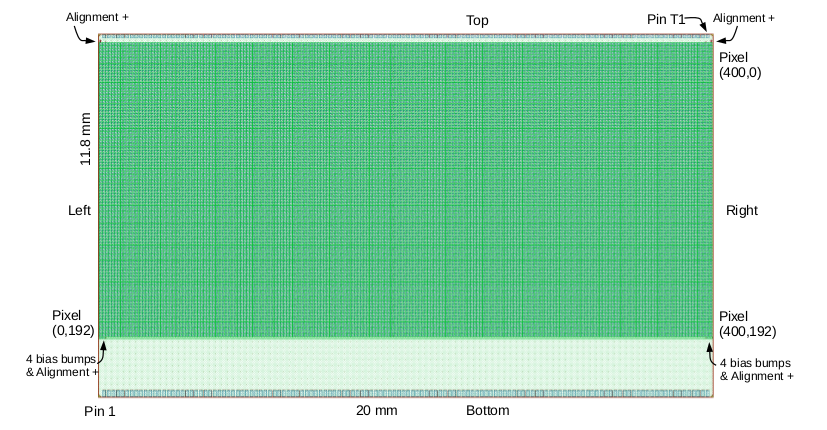
\includegraphics[scale=.4]{Immagini/RD53ALayout}
\caption{RD53A layout. Il chip è largo 20mm per 400 pixel e l'altezza è 11.8 mm per 192 pixel.}
\label{RD53ALayout}
\end{figure}

Facendo riferimento alla figura \ref{RD53ALayout}, l'area del chip che sarà saldata col sensore è posta nella parte alta ed è organizzata secondo una matrice di 192 $\times$ 400 pixel di area 50 $\mu$m $\times$ 50 $\mu$m.
Al di sopra di questa è presente una fila di \textit{pad} utilizzate per \textit{debug}, che sarà eliminata nella versione finale.
La parte di circuito necessaria per configurare, monitorare e leggere il chip, invece, si trova nella parte in basso con posta al di sotto solo una fila di pad per i \textit{wire-bond}. 
La matrice di pixel è organizzata in \textit{cores} di 8 $\times$ 8 pixel, all'interno di ciascuno dei quali i 64 front end sono disposti in gruppi di 4, chiamati isole analogiche, come mostrato in figura \ref{AnalogIsland}. 
Queste isole sono circondate da un ``mare'' digitale ed il circuito intorno ad ogni isola analogica non è lo stesso, ma cambia a seconda delle esigenze di progetto. 

\begin{figure}
\centering
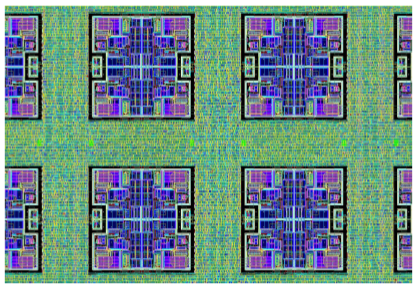
\includegraphics[scale=.5]{Immagini/AnalogIsland}
\caption{Immagine al microscopio della disposizione in "isole" dei \textit{front end}.}
\label{AnalogIsland}
\end{figure} 
Nelle parti più esterne del chip tutti i blocchi analogici sono raggruppati in macro blocchi chiamati Analog Chip Bottom (ACB).
Il blocco ACB è circondato dal blocco Digital Chip Bottom (DCB) che implementa la logica digitale per Input, Output e configurazione. 

\section{Front End}

Come detto in precedenza, RD53A, non è il chip finale, ma un prototipo al cui interno sono presenti tre differenti Front End per la parte analogica.
Si tratta di tre progetti diversi sono indicati con i nomi Sincrono, Lineare e Differenziale, vedi figura \ref{FrontEnd}. 
%Questi tre circuiti sono stati progettati da tre differenti gruppi e tra di loro ci sono importanti differenze.

Il FE Sincrono sfrutta un sistema di \textit{auto-zeroing} della linea di base, campionandola periodicamente, invece di aggiustare la soglia pixel per pixel. 
Il FE Lineare, invece, utilizza un amplificatore lineare all'ingesso del comparatore, che confronta il segnale con la soglia impostata. 
Il FE Differenziale ha uno stadio di guadagno differenziale all'ingresso del discriminatore. % e sbilanciando i due canali implementa la soglia.
Le caratteristiche comuni ai tre FE, invece, sono le piazzole per i bump-bond, il layout, la rete di polarizzazione per il sensore ed il circuito per iniettare segnali di calibrazione.
Questi ultimi due permettono un miglior confronto fra le prestazioni dei FE.
Inoltre, i tre FE condividono l'area del sensore e, dato che la matrice è larga 400 pixel ed è suddivisa in core da 8 $\times$ 8 pixel, non è possibile avere una egual area per i tre, ma due avranno 17 core per riga ed uno solo 16.
I FE Lineare e Differenziale sono stati posti accanto in quanto hanno funzionalità simili e metterli vicino consente di avere un'area con una risposta più uniforme anche in termini di consumi. 
\begin{figure}
\centering
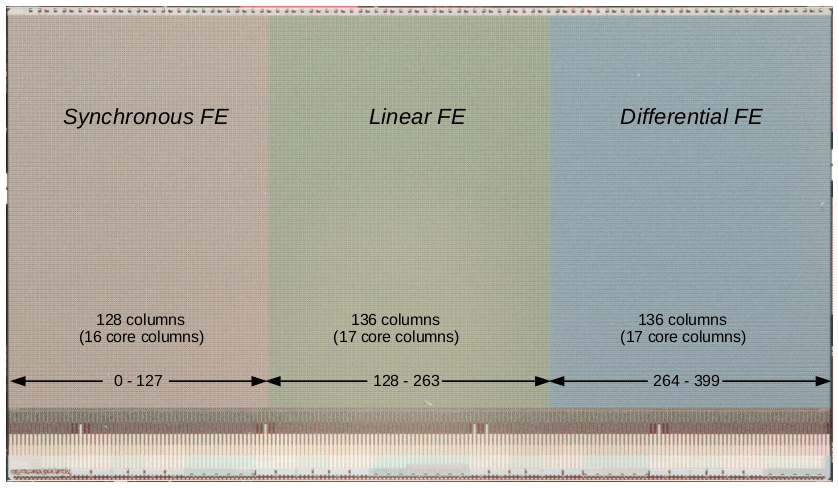
\includegraphics[scale=.3]{Immagini/FrontEnd}
\caption{Disposizione dei tre differenti \textit{front end} rispetto alla matrice di pixel 192 $\times$ 400.}
\label{FrontEnd}
\end{figure}

Descriviamo ora brevemente il funzionamento di ciascuno dei tre Front End:

\begin{itemize}

\begin{figure}
\centering
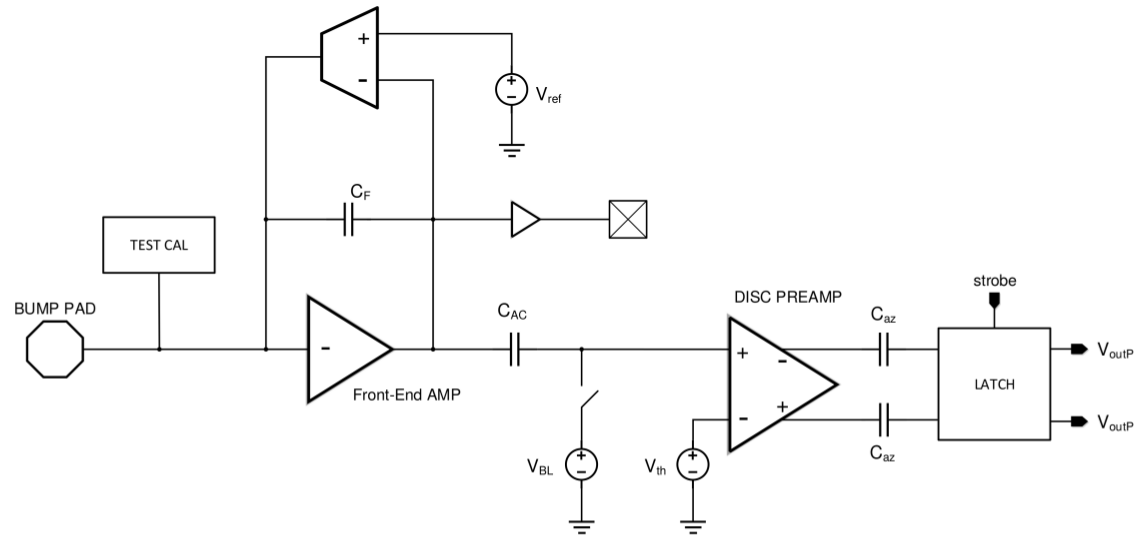
\includegraphics[width=\textwidth]{Immagini/SchemaSincrono}
\caption{Schematico del \textit{front end} Sincrono.}
\label{SchemaSincrono}
\end{figure}
\item \textbf{Sincrono}. Uno schema a blocchi del front end Sincrono è riportato in figura \ref{SchemaSincrono}. 
Questo consta di un amplificatore di carica (\textit{Charge Sensitive Amplifier} o CSA) a stadio singolo con un Krummenacher feedback accoppiato in AC ad un discriminatore sincrono, formato da un amplificatore differenziale e un latch di feedback positivo. 
Il Krummenacher feedback è progettato in modo da compensare sia la corrente dispersa dal sensore sia la corrente di scarica della capacità presente nell'anello di reazione. 
Maggiore la corrente maggiore la velocità del segnale del pre amplificatore a tornare al valore di \textit{baseline}. 
Si tenga presente, come riferimento, che una carica di di 10k$e^{-}$ e che produce 10 nA di corrente e un segnale di 400 ns viene ridotta ad un segnale di 40 nA di corrente di 100 ns.  
Inoltre, al fine di avere due differenti valori di guadagno, ci sono due capacità, rispettivamente di 2.5 fF e 4 fF. 
A causa di piccole differenze, che diventano rilevanti a scale di 65 nm, si hanno fluttuazioni della \textit{baseline} in uscita dal primo stadio dell'ordine delle decine di millivolt tra canali differenti.
Per questo motivo si è reso necessario un accoppiamento in AC al discriminatore. 
In ogni caso le differenze tra transistor si traducono in un offset della tensione in uscita dal discriminatore tra i vari pixel. 
Questo effetto, normalmente, è compensato con DAC locali che permettono regolazioni fini. Nel FE Sincrono, invece, l'offset è compensato attraverso un meccanismo di auto azzeramento (\textit{auto zeroing}). 
Per fare ciò è necessaria l'acquisizione del livello di tensione della \textit{baseline} ogni 100 $\mu$s o meno.
Durante le collisioni, la differenza tra segnale e baseline è inviata ad uno stadiodi confronto che genera il segnale di uscita del discriminatore.

\begin{figure}
\centering
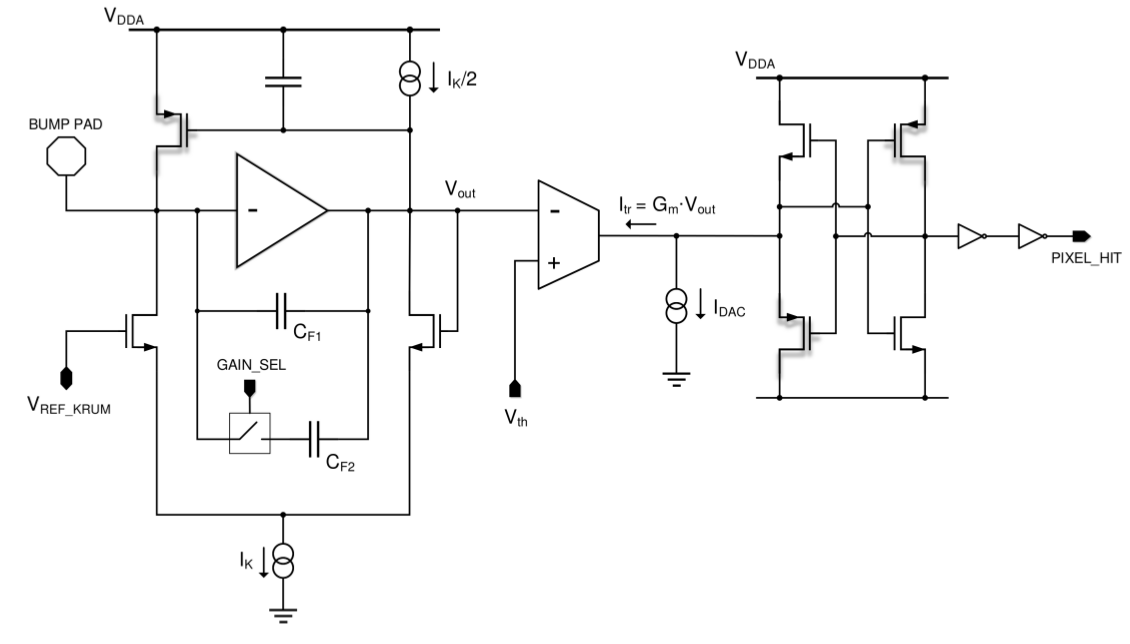
\includegraphics[width=\textwidth]{Immagini/SchemaLineare}
\caption{Schematico del \textit{front end} Lineare.}
\label{SchemaLineare}
\end{figure}
\item \textbf{Lineare}. Il front end lineare è mostrato in figura \ref{SchemaLineare}.
  Il circuito di lettura include un amplificatore di carica con un Krummenacher feedback per far fronte all'aumento di corrente di dispersione indotta dagli alti livelli di radiazione attesa. 
La scelta di un amplificatore a stadio singolo è dettata dai limiti sui consumi e sullo spazio disponibile all'interno del chip. 
Il segnale ottenuto dall'amplificatore di carica è mandato ad un comparatore che, insieme al contatore ToT (\textit{Time over Threshold}), è utilizzato per fare la conversione a segnale digitale. 
Gli aggiustamenti della tensione di soglia sono gestiti, canale per canale, da un circuito locale basato su un \textit{binary weighted} DAC, a 4 bit, che genera una corrente $\mathrm{I_{DAC}}$, fornendo una regolazione locale della soglia. 
Questo tipo di front end è stato ottimizzato per una carica massima di 30000 elettroni e un consumo complessivo di circa 4 $\mu$A. 
L'amplificatore può essere utilizzato in regime di alto o basso guadagno, modificando il bit GAIN$\_$SEL, mentre la corrente di recupero, $\mathrm{I_K}$/2, proveniente dal circuito di Krummenacher feedback, può essere configurata tramite un DAC. 
In configurazione di alto guadagno, per un segnale di carica pari a 30000, elettroni si ha un ToT di circa 400 ns, risultante in una corrente $\mathrm{I_K}$ di 25 nA. 
La risoluzione attesa è di 15 mV/k$e^{-}$, mentre diventa di 7.5 mV/k$e^{-}$ in configurazione di basso guadagno. 
Le prestazioni del preamplificatore di carica sono determinate, principalmente, dall'ingresso dell'amplificatore di carica e dalla parte del circuito di feedback con transistor PMOS. Dalle simulazioni il rumore in carica equivalente, per un rivelatore con capacità di 50 fF, è di 87 elettroni e, dopo la messa a punto, la dispersione della soglia scende da 380 a 35 elettroni.
%Da simulazioni la dispersione della soglia dovrebbe passare da 380 elettroni a 35 elettroni dopo la messa a punto.

\begin{figure}
\centering
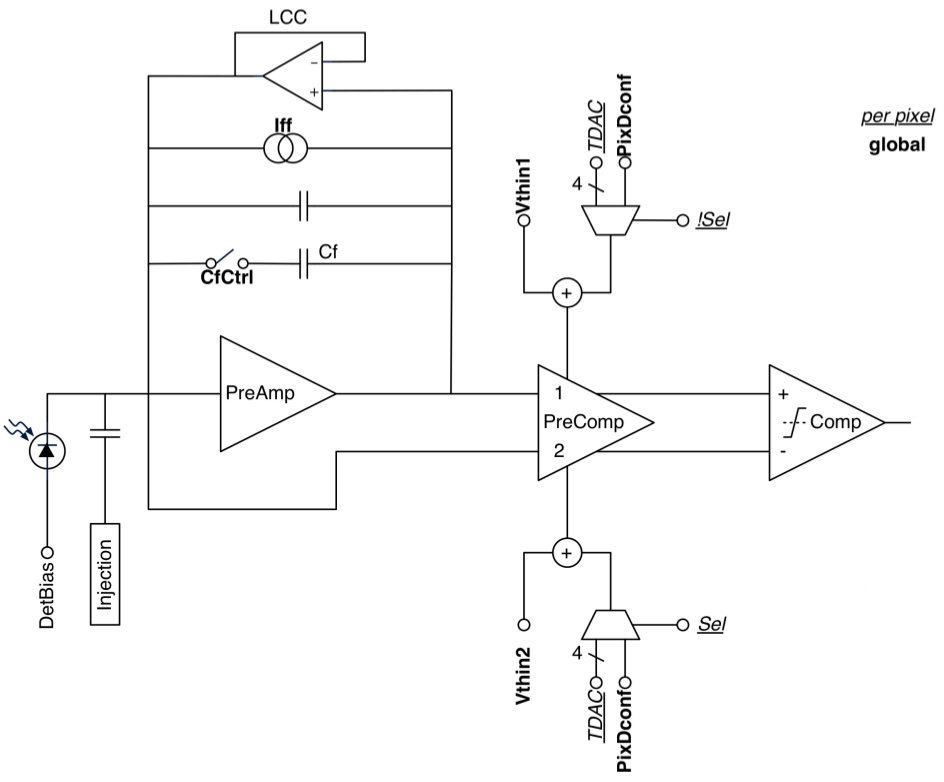
\includegraphics[scale=.3]{Immagini/SchemaDifferenziale}
\caption{Schematico del \textit{front end} Differenziale.}
\label{SchemaDifferenziale}
\end{figure}
\item \textbf{Differenziale}. Il front end Differenziale è un circuito puramente analogico: non ha al suo interno latches, flip-flop o contatori. 
I valori di configurazione sono, però, forniti da un nucleo digitale, che riceve dalla parte analogica solo il segnale in uscita del comparatore. 
Naturalmente è necessaria la presenza di un ADC per la digitalizzazione del ToT ottenuto dal comparatore, anch'esso implementato interamente nella parte digitale. 
Lo schema a blocchi del front end differenziale è riportato in figura \ref{SchemaDifferenziale}. 
Il pre amplificatore, presente nel primo stadio, ha un guadagno continuo, regolabile tra i due valori di capacità presenti nell'anello di reazione.
Il feedback in corrente è impostabile globalmente e non può essere regolato su ogni singolo pixel. 
Dalle misure sui prototipi è stato visto che la dispersione nei valori di ToT che ne consegue ha un livello accettabile anche senza la necessità di una pre regolazione.  
In caso di assenza di segnale, il feedback assicura che input e output del preamplificatore siano allo stesso potenziale.
Nel secondo stadio, il pre comparatore fornisce un guadagno aggiuntivo e agisce come soglia differenziale.
La soglia globale può essere regolata tramite le tensioni VTH1 e VTH2, mentre localmente la soglia è modificata utilizzando un \textit{resistor ladder} a 4 bit in ciascuno dei due rami del pre comparatore.
Oltre ai 4 bit ce n'è un quinto che seleziona il ramo da modificare. 
Dopo il pre comparatore si ha uno stadio con un comparatore, la cui uscita è collegata alla regione digitale tramite porte logiche. 
Progettato per operare con una soglia di 500 elettroni, la parte analogica ha un consumo di 4$\mu$A/pixel, considerando una capacità di 50 fF e 10 nA di corrente dispersa.

\end{itemize}

\section{Alimentazione}
\begin{figure}
\centering
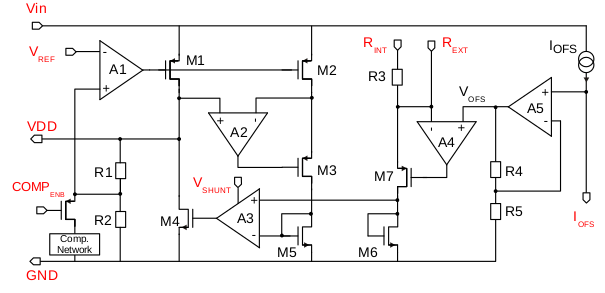
\includegraphics[width=\textwidth]{Immagini/SLDO_RD53A}
\caption{Regolatore LDO con Shunt (Shunt-LDO).}
\label{SLDO_RD53A}
\end{figure}
In RD53A l'alimentazione è gestita da due regolatori LDO con shunt, uno per la parte analogica ed uno per quella digitale. 
Rispetto al circuito di SLDO presentato in precedenza, la tensione di offset è generata con un circuito diverso.
Lo schema del circuito di SLDO è riportato in  figura \ref{SLDO_RD53A}, mentre i valori di Input e Output sono riportati nella seguente tabella:

%\begin{center}
\begin{small}
\noindent\setlength\tabcolsep{4pt}%
\begin{tabularx}{\linewidth}{|c|c|c|c|c|X|}
%\begin{tabular}{|c|c|c|c|c|l|}
\hline
\textbf{Pin} & \textbf{Tipologia} & \textbf{Min} & \textbf{Tipico} & \textbf{Max} & \textbf{Descrizione} \\ \hline

$\mathrm{V_{IN}}$ & Alimentazione & 1.4 V & & 2.0 V & Input di alimentazione esterna (in tensione)\\ \hline
 & Power & 0 A & 0.5 A & 2.0 A & Input di alimentazione esterna (in corrente)\\ \hline     
$\mathrm{V_{SHUNT}}$ & Alimentazione & 1.4 V & & 2.0 V & Tensione di alimentazione per il circuito di shunt\\ \hline
GND & Ground &  & &  & Terra locale e uscita della corrente di shunt\\ \hline
VDD & Alimentazione & 1.0 V & 1.2 V & 1.32 V & Tensione di uscita del regolatore\\ \hline
$\mathrm{V_{REF}}$ & Analogico & 500 mV & 600 mV & 660 mV & Tensione di riferimento (VDD=2$\mathrm{V_{REF}}$)\\ \hline
$\mathrm{R_{INT}}$ & Analogico &  & $\mathrm{V_{IN}}$ &  & Abilita la resistenza interna R\\ \hline
$\mathrm{R_{EXT}}$ & Analogico & 300 $\Omega$ &  &  & Resistenza esterna collegata a $\mathrm{V_{IN}}$\\ \hline
$\mathrm{I_{OFS}}$ & Analogico &  & 200 k$\Omega$ &  & Resistenza esterna connessa a GND\\ \hline
$\mathrm{COMP_{ENB}}$ & Digitale &  & GND &  & Segnale per abilitare il circuito di compensazione\\ \hline
\end{tabularx}
\end{small}
%\end{center}

Il valore di $\mathrm{V_{ofs}}$ è determinato dalla caduta di tensione sulla resistenza applicata al terminale $\mathrm{I_{ofs}}$ e che va saldata nell'apposito slot della Single Chip Card.
Il valore di $\mathrm{I_{ofs}}$ è 2 $\mu$A, dunque:
\begin{equation}
\label{eq:Vofs}
\mathrm{V_{ofs} = 2 \mu A \cdot R_{iofs}}
\end{equation}
Questa tensione viene raddoppiata tramite l'azione dell'anello di reazione di A5, prima di essere mandata ad A4.
Il comportamento della tensione in ingresso sarà:
\begin{equation}
\mathrm{V_{in}= 2 \cdot V_{iofs} + \dfrac{R3}{1000} \cdot I_{in}}
\end{equation}
Le misure presentate nelle sezioni successive sono stati ottenuti con i seguenti valori di R3 e $\mathrm{V_{ofs}}$:

\begin{center}
\begin{tabular}{lc}
\hline
$\mathrm{R3}$ & 600 $\Omega$ \\%misurata con il multimetro è 620
$\mathrm{R_{iofs}}$ & 250 k$\Omega$\\ 
\hline
\end{tabular}
\end{center}
Dall'equazione \ref{eq:Vofs}, una $\mathrm{R_{iofs}}$ di 250 k$\Omega$ corrisponde ad una tensione di offset di circa 0.5 V.
Nell'andamento della tensione in ingresso in funzione della corrente, quindi, ci aspettiamo un valore misurato per l'offset di circa 1 V.

Per quanto riguarda le tensioni di riferimento, come $\mathrm{V_{ref}}$, queste vengono generate all'interno del chip da un circuito dedicato, in cui si utilizzano bandgap.
Il valore di uscita dei bandgap è configurabile e di default è 16, corrispondente a una tensione di circa 1.15 V, variando leggermente da un chip all'altro.
Un esempio è quello di figura \ref{bandgap_trimming}, in cui sono riportati gli andamenti misurati di $\mathrm{V_{ref}}$ al variare del valore di configurazione, per differenti chip.

\begin{figure}
\centering
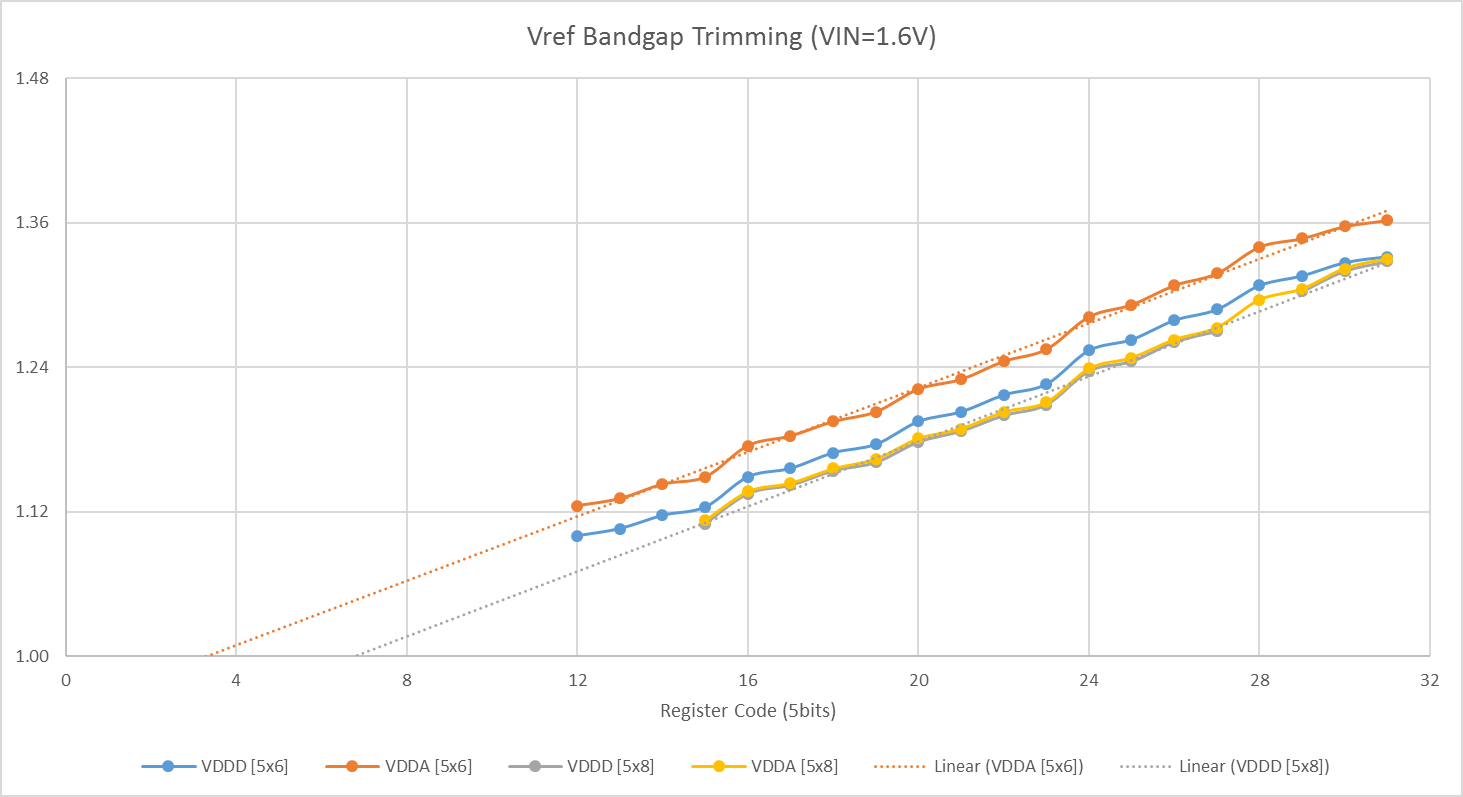
\includegraphics[scale=.5]{Immagini/bandgap_trimming}
\caption{Andamento della tensione di $\mathrm{V_{ref}}$ generata internamente, per due diversi chip, al variare del parametro di configurazione, il valore di default è 16.}
\label{bandgap_trimming}
\end{figure}

\section{Single Chip Card}

Analogamente a quanto visto per gli SLDO, che vengono collaudati usando una PCB di test, per il chip RD53A è necessario l'utilizzo di una SCC (\textit{Single Chip Card}). 
Il chip è fissato al centro di questa scheda e, attraverso \textit{wire bond}, è connesso ai vari elementi della scheda (pin di monitoraggio, molex di alimentazione, DisplayPort per la trasmissione/ricezione di dati, jumper per la configurazione, etc...). 
Il chip viene montato sulla scheda in un apposito spazio, ai cui bordi arrivano le varie piste da connettere e sotto cui, al posto della vetronite, c'è uno spessore metallico con via termici che permettono l'applicazione di un sistema refrigerante sulla parte posteriore della SCC. 
Nel momento in cui l'alimentazione del chip viene fornita dai due SLDO, infatti, la corrente non utilizzata viene dissipata sui due shunt, che si scaldano rendendo, quindi, necessario un sistema di raffreddamento.
%La presenza di un raffreddamento è necessaria nel momento in cui l'alimentazione è data utilizzando i due SLDO, infatti, la corrente non necessaria al chip viene dissipata sui due shunt che diventano punti molto caldi. 
Al fine di evitare danneggiamenti del chip, e dell'eventuale sensore collegato, questo va raffreddato utilizzando dissipatori di calore. 

Dal momento che il chip è un prototipo si è lasciata la possibilità di configurare l'alimentazione esternamente, scegliendo tra tre diverse configurazioni.
Inoltre è possibile mantenere separate, a livello di alimentazione, la regione digitale e quella analogica
\footnote{
Nel chip finale gli ShuntLDO della parte digitale e analogica saranno in parallelo.
}.
Le possibili configurazioni sono:

\begin{itemize}
\begin{figure}
\centering
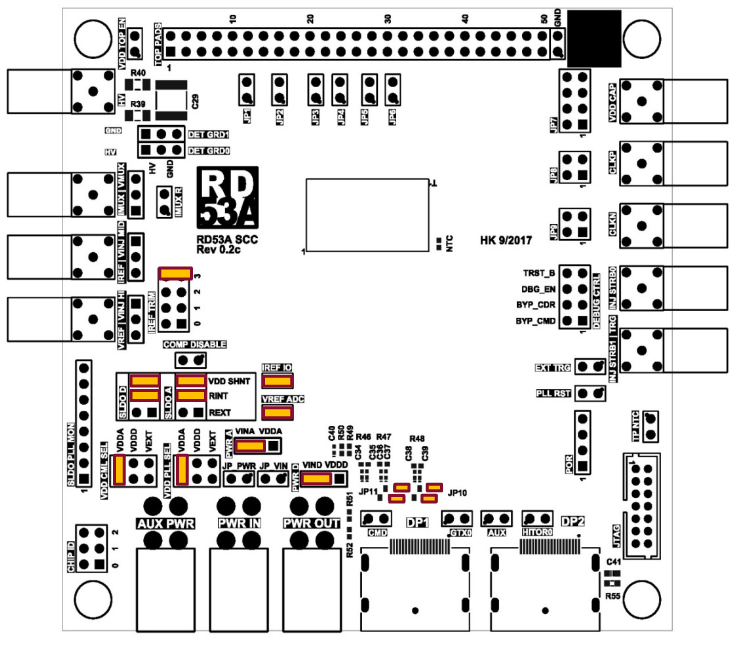
\includegraphics[scale=.3]{Immagini/SLDOmode}
\caption{Configurazione dei jumper per l'utilizzo di RD53A alimentato attraverso il circuito di ShuntLDO, sia per la regione analogica sia per quella digitale.}
\label{SLDOmode}
\end{figure}
\item Alimentazione attraverso il circuito di ShuntLDO. In questo caso il generatore utilizzato sarà in corrente e sulla SCC card la configurazione dei jumper sarà quella riportata in figura \ref{SLDOmode}. 
Per operare con il chip in configurazione SLDO è necessario l'utilizzo di un sistema di raffreddamento per il chip che, in normali condizioni di lavoro, può essere un semplice dissipatore passivo.
Nella misura delle varie tensioni, però, l'effetto di deriva termica non è trascurabile e, quindi, è meglio utilizzare un sistema di raffreddamento attivo, con un buon contatto termico e che permetta di controllare le temperature, come, ad esempio, si può ottenere con l'impiego di peltier.

\begin{figure}
\centering
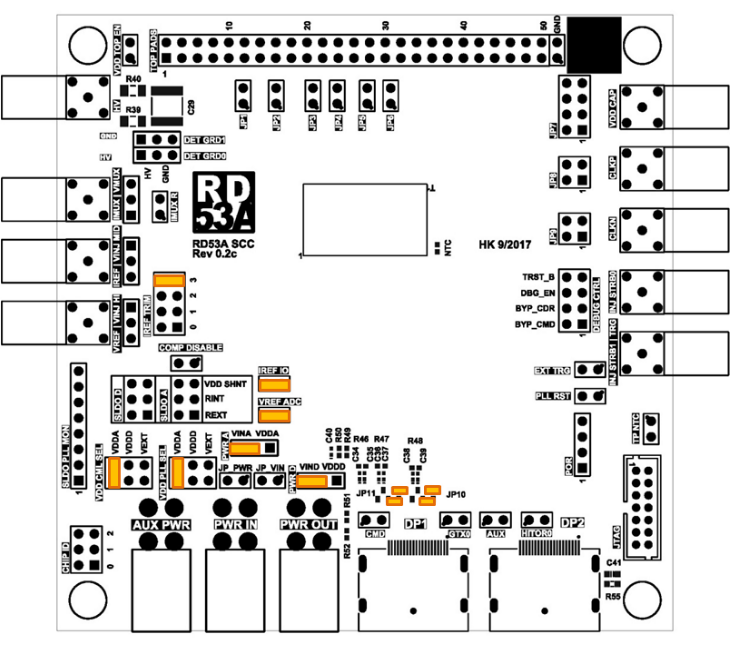
\includegraphics[scale=.3]{Immagini/LDOmodeDefault}
\caption{Configurazione dei jumper per l'utilizzo di RD53A alimentato dal regolatore LDO senza la parte di shunt.}
\label{LDOmode}
\end{figure}
\item Alimentazione senza Shunt, utilizzando solo il regolatore LDO.
  Questa configurazione necessita di una alimentazione in tensione e sarà il generatore esterno a dover fornire più o meno corrente in relazione ai consumi del chip.
  L'utilizzo del solo regolatore permette di avere un consumo minimo in termini di potenza e, dunque, di operare con il chip senza il bisogno di un sistema di raffreddamento.
  In questo caso la configurazione dei jumper è quella riportata in figura \ref{LDOmode}.

\begin{figure}
\centering
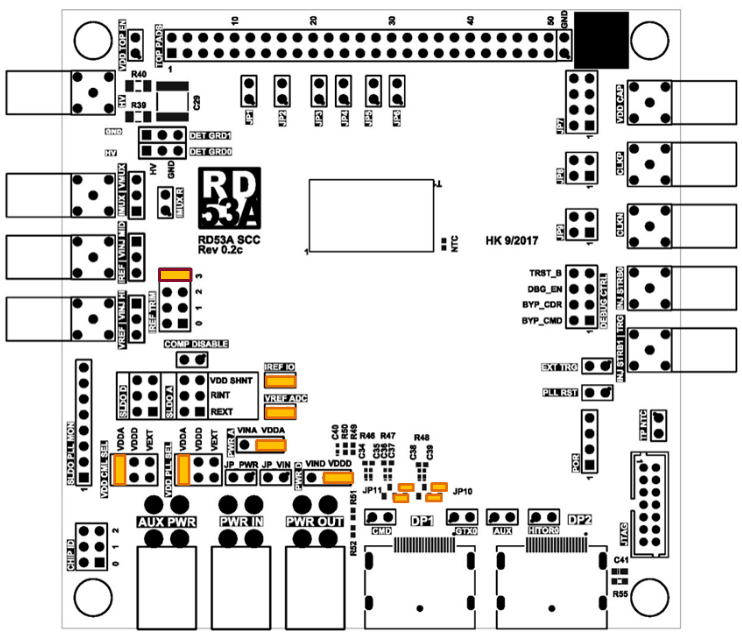
\includegraphics[scale=.3]{Immagini/DirectPowering}
\caption{Configurazione dei jumper per l'utilizzo di RD53A alimentato direttamente, escludendo il circuito di ShuntLDO.}
\label{DirectPowering}
\end{figure}
\item Alimentazione diretta.
  Il circuito con regolatore e shunt viene completamente escluso ed il chip è alimentato direttamente dal generatore di tensione. 
Questa configurazione è riportata in figura \ref{DirectPowering}.
L'utilizzo dell'alimentazione diretta è delicato per varie ragioni, fra cui il più importante è il rischio di danneggiamento di RD53A. 
La presenza del regolatore LDO, anche privo di shunt, assicura che sbalzi di tensione all'ingresso dell'alimentazione non siano trasmessi al chipi ed, inoltre, il regolatore può sopportare tensioni fino a 2 V, mentre il chip già sopra 1.32 V rischia di danneggiarsi. L'esclusione di questa sicurezza con la scelta di utilizzare un'alimentazione diretta è, perciò, sconsigliata. 
\end{itemize}

\section{Misure Statiche con RD53A}

Utilizzando il chip in configurazione ShuntLDO, raffreddato in modo passivo con un radiatore a contatto termico con il retro, si è proceduto alla caratterizzazione statica del comportamento dei due circuiti di alimentazione presenti nel chip
\footnote{
  Uno per la parte analogica ed uno per quella digitale.
}.
Questa caratterizzazione è stata effettuata con diverse configurazioni, che possono essere riassunte nella scelta dei seguenti tre punti:
%Nel far questo sono state scelte diverse configurazioni, le scelte principali possono essere riassunte in tre punti:
\begin{itemize}
  \item Alimentazione dei due regolatori con SLDO: indipendenti o in parallelo fra loro.
  \item Rampa di corrente: crescente o decrescente.
  \item Tensioni di riferimento $\mathrm{V_{ref}}$ e $\mathrm{V_{iofs}}$: generate internamente o fornite dall'esterno.
%\item Tenere i due regolatori con SLDO in parallelo o con alimentazione indipendenti.
%\item Variare la corrente partendo da 0 A incrementandola via via o partendo da 1.5 A andando poi a decrescere.
%\item Utilizzare $\mathrm{V_{ref}}$ e $\mathrm{V_{iofs}}$ generati internamente o fornirli esternamente.
\end{itemize}

Nella seguente tabella è riportata la descrizione delle abbreviazioni utilizzate per le legende dei grafici:

\begin{center}
%\noindent\setlength\tabcolsep{4pt}%
\begin{tabularx}{\linewidth}{|cc|X|}
\hline
\multicolumn{2}{|c|}{Abbreviazione} & \multicolumn{1}{c|}{\multirow{2}{*}{Segnale}}\\ 
Analogico & Digitale & \\
\hline
VINA & VIND & Tensione all'ingresso del regolatore  \\ \hline
VDDA & VDDD & Tensione in uscita (alimentazione chip) \\ \hline
$\mathrm{V_{iofs \_ m \_ A}}$ & $\mathrm{V_{iofs \_ m \_ D}}$ & Tensione riferimento offset (va raddoppiata) \\ \hline   
$\mathrm{V_{ref \_ m \_ A}}$ & $\mathrm{V_{ref \_ m \_ D}}$ & Tensione riferimento per VDDA e VDDD (va raddoppiata)\\ \hline   
\end{tabularx}
\end{center}

\subsubsection{Alimentazioni indipendenti, rampa di corrente crescente, tensioni di riferimento interne}

\begin{figure}
\centering
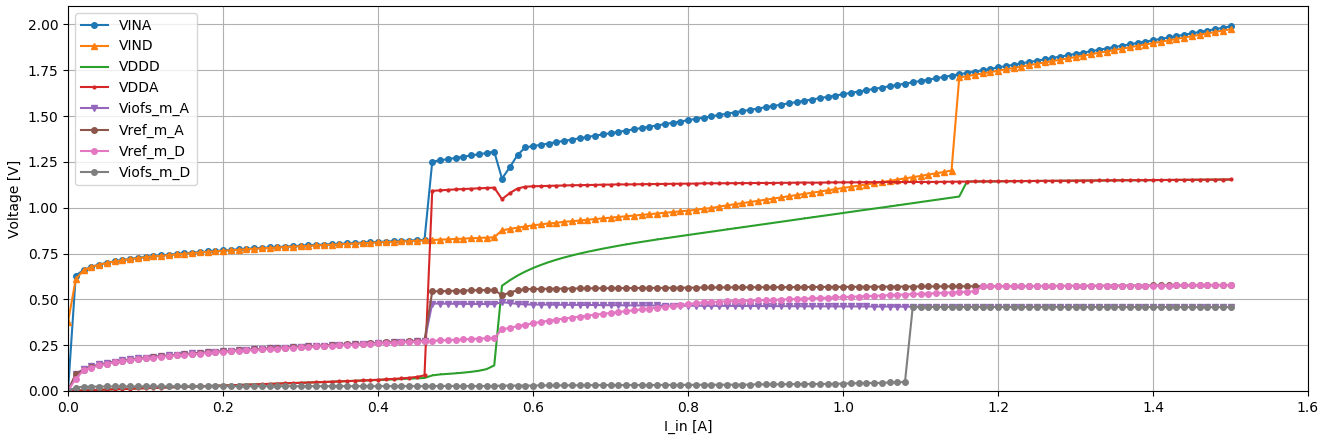
\includegraphics[width=\textwidth]{Immagini/IUI2}
\caption{Grafico corrente-tensione ottenuto tenendo i due regolatori separati e variando la corrente da 0 A a 1.5 A.}%allungare descrivendo anche l'undershoot
\label{IUI}
\end{figure}
Le prime misure sono state eseguite utilizzando, come riferimento per $\mathrm{V_{out}}$ e $\mathrm{V_{iofs}}$, le tensioni generate internamente al chip.
La corrente fornita ai due SLDO, alimentati indipendentemente, è stata variata, contemporaneamente, da 0 A a 1.5 A, a passi di 10 mA.
L'andamento ottenuto è quello riportato in figura \ref{IUI}.

L'undershoot ben visibile sulla tensione, in ingresso e in uscita, della parte analogica è causato da una distribuzione non uguale delle correnti nei due SLDO: quando si attiva la parte digitale si ha un picco di assorbimento di corrente, che causa un drop nella parte analogica, la cui entità è descritta dalla seguente tabella:
\begin{center}
\begin{tabular}{ccc }
\hline
$\Delta \mathrm{V_{INA}}$ & $\Delta \mathrm{V_{DDA}}$ &$\Delta \mathrm{V_{DDA}}$  \\ \hline
$\sim$0.150 V & $\sim$ 0.030 V& $\sim$0.060 V\\ \hline     
\end{tabular}
\end{center}
Questo fenomeno è stato osservato nonostante la configurazione sia tale da avere i due SLDO, per la parte digitale e analogica, alimentati separatamente, segno che, all'interno del chip, sono presenti delle zone di ``dialogo'' fra i due: un po' di corrente scorre attraverso le connessioni tra le due regioni, causando la caduta di tensione della parte analogica osservata.
%Questo avviene nonostante le alimentazioni dei due SLDO siano separate, in quanto all'interno del chip ci sono zone di 'dialogo' tra regione analogica e digitale. 
%Si ha scorrimento di corrente attraverso connessioni tra le due regioni che causano cadute di tensioni nella parte analogica, questo comportamento è pericoloso e va evitato. 
Questo comportamento è pericoloso e va evitato.

Inoltre, sempre dalla figura \ref{IUI}, si può notare che la parte digitale si attiva a un valore di $\mathrm{I_{in}}$ di 0.56 A, non riuscendo però ad andare a regime, poiché la tensione in ingresso non è abbastanza alta da consentire un corretto funzionamento.
Questo è dovuto al ritardo con cui il $\mathrm{V_{iofs}}$ digitale arriva al valore corretto.
Infatti, come introdotto in precedenza, la tensione di riferimento dell'offset è ottenuta dalla caduta di tensione su una resistenza, nel nostro caso di $\sim$250 k$\Omega$, data dal passaggio di una corrente di 2 $\mu$A.
Se, per vari motivi, il circuito che genera questa corrente ha un ritardo nell'accensione, questo si ripercuote nell'accensione del chip.  
Tutti questi problemi sono legati all'accensione e, quindi, dovranno scomparire con uno scan eseguito partendo da valori alti di corrente per poi scendere fino a 0 A.

%\begin{center}
%\begin{tabular}{|l|c|c|c|c|}
%\hline
% & \multicolumn{2}{c|}{Digitale} & \multicolumn{2}{c|}{Analogica} \\ \hline
% 
%& media & errore & media & errore \\ \hline
%
%$\mathrm{R_{eq}}$ & 0.752 $\Omega$ & 0.0003 $\Omega$& 0.7178 $\Omega$ & 0.0003 $\Omega$ \\ \hline
%$\mathrm{V_{ofs}}$ & 0.844 V& 0.004 V & 0.9025 V & 0.0003 V\\ \hline     
%
%\end{tabular}
%\end{center}

%\begin{figure}
%\centering
%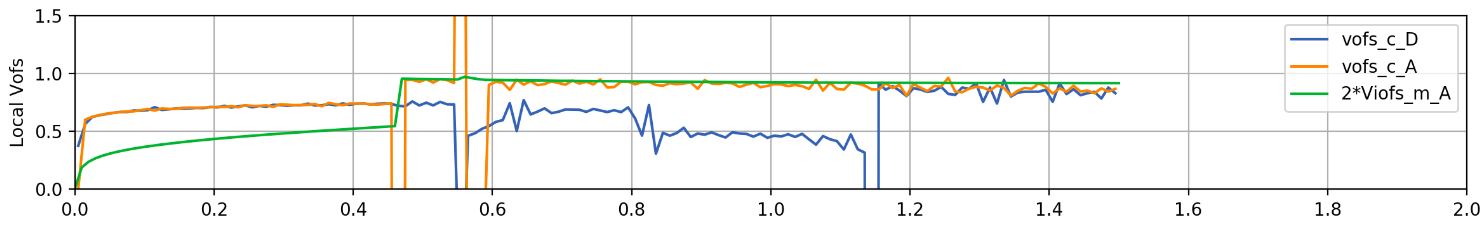
\includegraphics[scale=.27]{Immagini/IUISubPlotVofs}
%\caption{.}
%\label{IUISubPlotVofs}
%\end{figure}

%\begin{center}
%\begin{tabular}{|l|c|c|}
%\hline
%&Digitale  &Analogica \\ \hline
%$\mathrm{R_{eq}}$ & 0.753 $\Omega$& 0.724 $\Omega$ \\ \hline
%$\mathrm{V_{ofs}}$ & 0.845 V & 0.900 V\\ \hline
%\end{tabular}
%\end{center}

\subsubsection{Alimentazioni indipendenti, rampa di corrente decrescente, tensioni di riferimento interne}

\begin{figure}
\centering
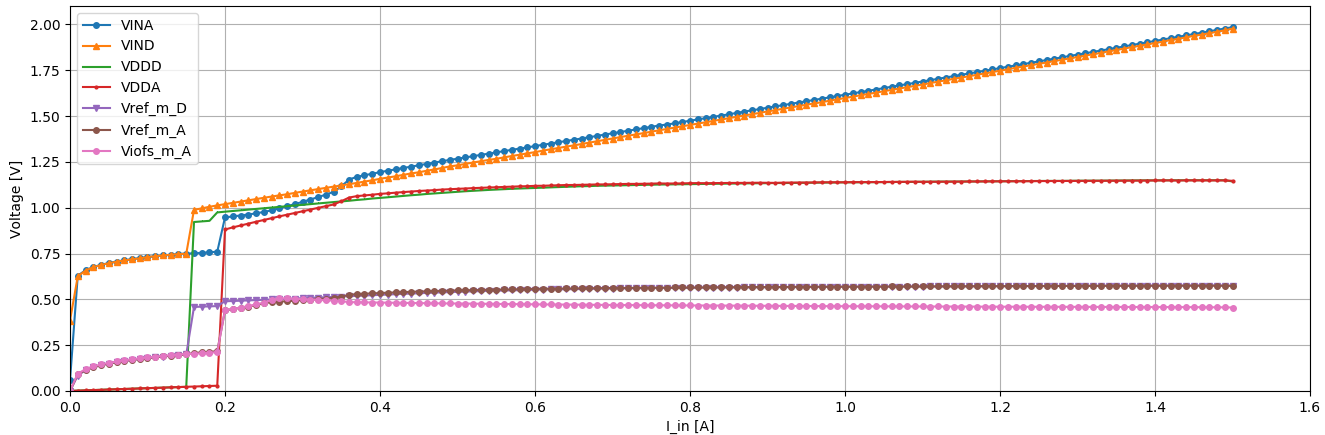
\includegraphics[width=\textwidth]{Immagini/IDI2}
\caption{Grafico corrente-tensione ottenuto tenendo i due regolatori separati e variando la corrente da 1.5 A a 0 A.}
\label{IDI}
\end{figure}

La seconda serie di misure, il cui andamento è riportato in figura \ref{IDI}, è stata ottenuta con la stessa configurazione del caso precedente, ma con rampa di corrente decrescente fra 1.5 A e 0A.
Dal grafico si può notare come gli undershoot, presenti nella precedente scansione, non siano più visibili, in accordo con la giustificazione data, cioè che siano dovuti all'attivazione del chip, che richiede consumi più elevati. 
Una volta che il chip ha raggiunto la configurazione di default, e finché non riceve un segnale di clock esterno, i consumi sono di circa 50 mA, per la parte digitale, e 400 mA, per quella analogica.
%Questo fin tanto che il chip non riceve un segnale di clock esterno. 
Questa differenza in consumi di corrente, tra parte analogica e digitale, si riflette nel fatto che, diminuendo ulteriormente la corrente, la prima regione a mostrare problemi è quella analogica, mostrando un primo flesso poco i sotto 400 mA e spegnendosi a 200 mA.
La parte digitale, invece, riesce a rimanere attiva anche con correnti inferiori a 200 mA. 
Inoltre, partendo da valori di corrente elevati, e quindi tensioni in ingresso ben al di sopra di quelle minime, non si osservano neppure i problemi dovuti ai differenti istanti di accensione di parte analogica e digitale.
%\begin{center}
%\begin{tabular}{|l|c|c|c|c|}
%\hline
% & \multicolumn{2}{c|}{Digitale} & \multicolumn{2}{c|}{Analogica} \\ \hline
% 
%& media & errore & media & errore \\ \hline
%
%$\mathrm{R_{eq}}$ & 0.73475 $\Omega$ & 0.00008 $\Omega$& 0.7153 $\Omega$ & 0.0006 $\Omega$ \\ \hline
%$\mathrm{V_{ofs}}$ & 0.86530 V& 0.00007 V & 0.9043 V & 0.0005 V\\ \hline     
%
%\end{tabular}
%\end{center}

Continuando a tenere i due circuiti di alimentazione separati è interessante studiare il comportamento ottenuto fornendo esternamente le varie tensioni di riferimento.

\subsubsection{Alimentazioni indipendenti, rampa di corrente crescente, $\mathrm{V_{ref}}$ esterna} 

\begin{figure}
\centering
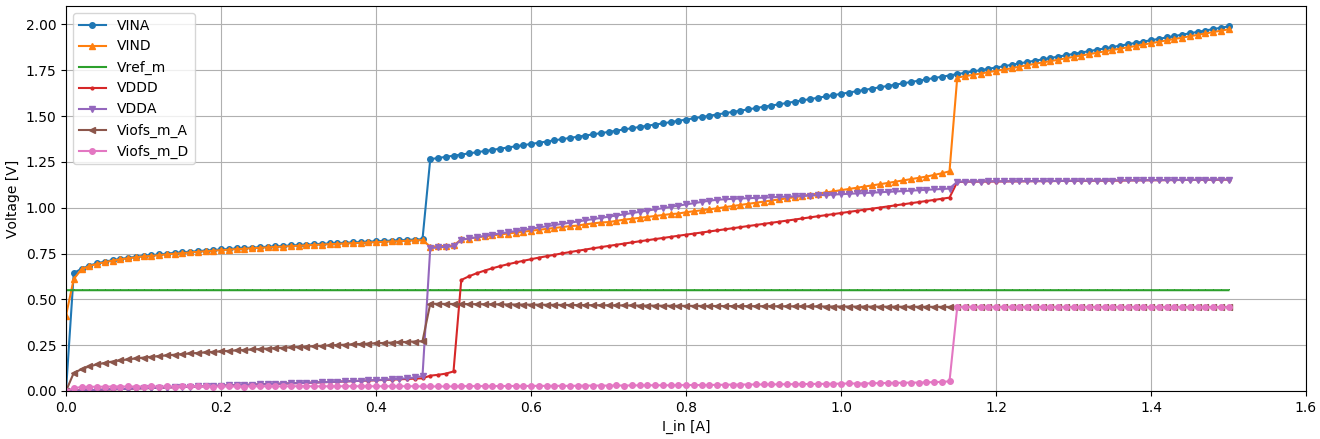
\includegraphics[width=\textwidth]{Immagini/IUEVref2}
\caption{Grafico corrente-tensione ottenuto tenendo i due regolatori separati e variando la corrente da 0 A a 1.5 A, utilizzando un riferimento esterno per $\mathrm{V_{ref}}=0.550 \V$.}
\label{IUEVref}
\end{figure}
Il grafico riportato in figura \ref{IUEVref} è ottenuto fornendo esternamente  $\mathrm{V_{ref}}=0.550 \V$,  sia per la parte analogica che per quella digitale.
Il comportamento della parte digitale è analogo a quello ottenuto nel primo grafico di figura \ref{IUI}, mentre, per la parte analogica, non si ha l'undershoot osservato in precedenza per $\mathrm{V_{INA}}$ e, dunque, nemmeno per $\mathrm{V_{DDA}}$.
Quest'ultima tensione, però, risente ancora del comportamento della parte digitale: fintantoché $\mathrm{V_{iofs\_ m \_ D}}$ non arriva al valore corretto $\mathrm{V_{DDA}}$ non si stabilizza.

%\begin{center}
%\begin{tabular}{|l|c|c|c|c|}
%\hline
% & \multicolumn{2}{c|}{Digitale} & \multicolumn{2}{c|}{Analogica} \\ \hline
% 
%& media & errore & media & errore \\ \hline
%
%$\mathrm{R_{eq}}$ & 0.7539 $\Omega$ & 0.00007 $\Omega$& 0.7448 $\Omega$ & 0.0002 $\Omega$ \\ \hline
%$\mathrm{V_{ofs}}$ & 0.84199 V& 0.00011 V & 0.8706 V & 0.0003 V\\ \hline     
%
%\end{tabular}
%\end{center}

\subsubsection{Alimentazioni indipendenti, rampa di corrente crescente, $\mathrm{V_{iofs}}$ esterna} 

\begin{figure}
\centering
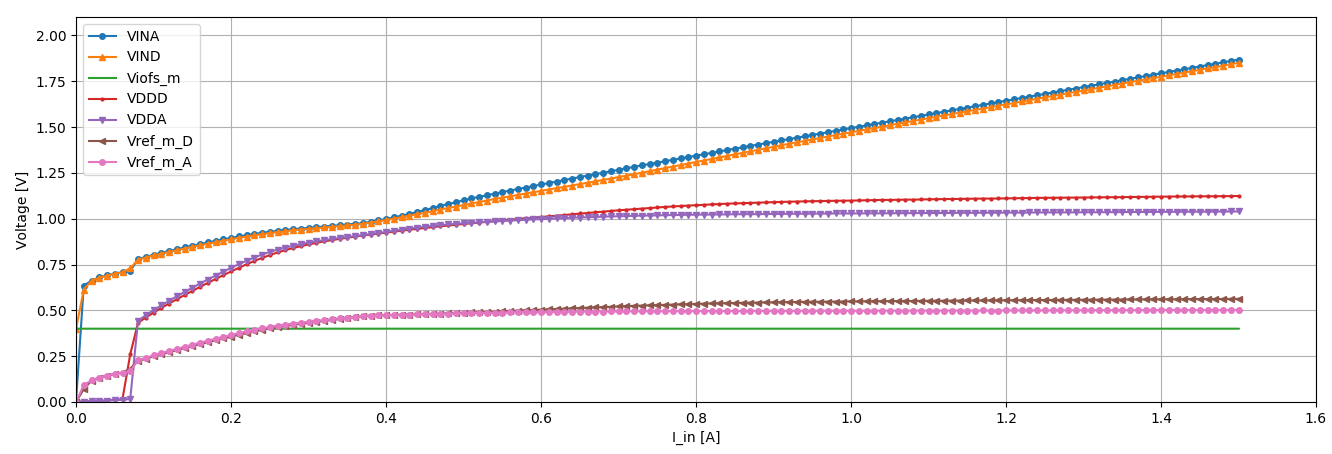
\includegraphics[width=\textwidth]{Immagini/IUEViofs2}
\caption{Grafico corrente-tensione ottenuto tenendo i due regolatori separati e variando la corrente da 0 A a 1.5 A, utilizzando un riferimento esterno per $\mathrm{V_{iofset}}=0.400 \V$.}
\label{IUEViofs}
\end{figure}
Le stesse misure sono state ripetute fornendo esternamente il solo $\mathrm{V_{iofset}}=0.400 \V$, utilizzando per $\mathrm{V_{ref}}$ quello interno e tenendo le alimentazioni dei due SLDO indipendenti. 
In questo caso gli andamenti ottenuti sono decisamente migliori come si vede in figura \ref{IUEViofs}. 
Infatti, il $\mathrm{V_{iofset}}$ esterno permette di evitare i problemi riscontrati in precedenza, quali il differente valore di attivazione di $\mathrm{I_{in}}$ tra parte analogica e digitale, poiché l'offset è al valore di riferimento giusto sin dall'inizio.
%\begin{center}
%\begin{tabular}{|l|c|c|c|c|}
%\hline
% & \multicolumn{2}{c|}{Digitale} & \multicolumn{2}{c|}{Analogica} \\ \hline
% 
%& media & errore & media & errore \\ \hline
%
%$\mathrm{R_{eq}}$ & 0.7871 $\Omega$ & 0.0013 $\Omega$& 0.7554 $\Omega$ & 0.0013 $\Omega$ \\ \hline
%$\mathrm{V_{ofs}}$ & 0.6824 V& 0.0013 V & 0.7403 V & 0.0012 V\\ \hline     
%
%\end{tabular}
%\end{center}

%\begin{figure}
%\centering
%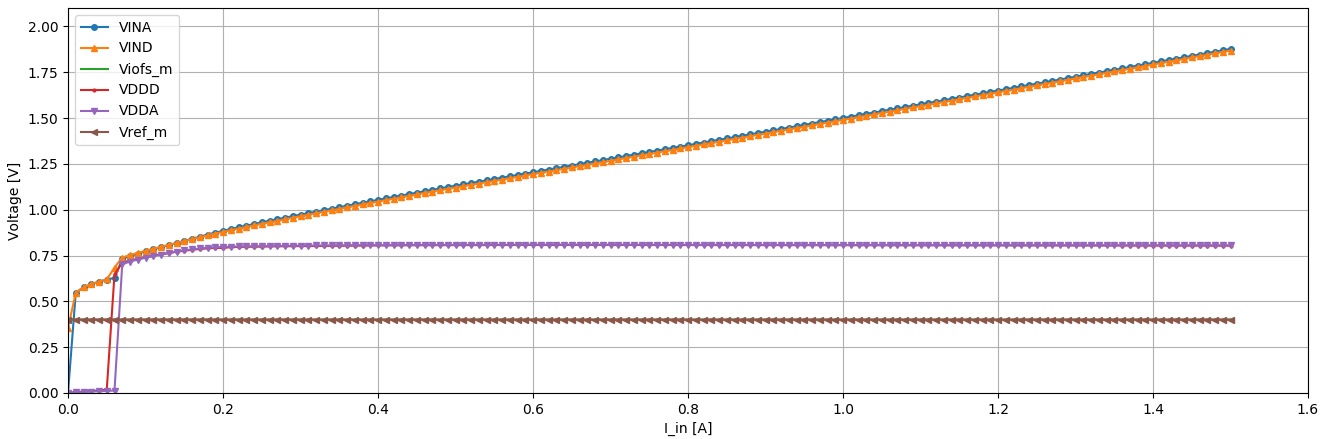
\includegraphics[scale=.3]{Immagini/IUEAll}
%\caption{IUEAll viofs e vref si sovrappongono .}
%\label{IUEAll}
%\end{figure} 
%Infine riportiamo il grafico degli andamenti nal caso in cui sia $\mathrm{V_{ref}}$ che $\mathrm{V_{iofset}}$ sono forniti esternamente. entrambi valgono 0.400, mancanza di kitley

%\begin{center}
%\begin{tabular}{|l|c|c|c|c|}
%\hline
% & \multicolumn{2}{c|}{Digitale} & \multicolumn{2}{c|}{Analogica} \\ \hline
% 
%& media & errore & media & errore \\ \hline
%
%$\mathrm{R_{eq}}$ & 0.7461 $\Omega$ & 0.0004 $\Omega$& 0.7448 $\Omega$ & 0.0004 $\Omega$ \\ \hline
%$\mathrm{V_{ofs}}$ & 0.7452 V& 0.0004 V & 0.7563 V & 0.0004 V\\ \hline 
%\end{tabular}
%\end{center}  

\subsubsection{Alimentazione in parallelo, rampa di corrente crescente, tensioni di riferimento interne} 

\begin{figure}[h]
\centering
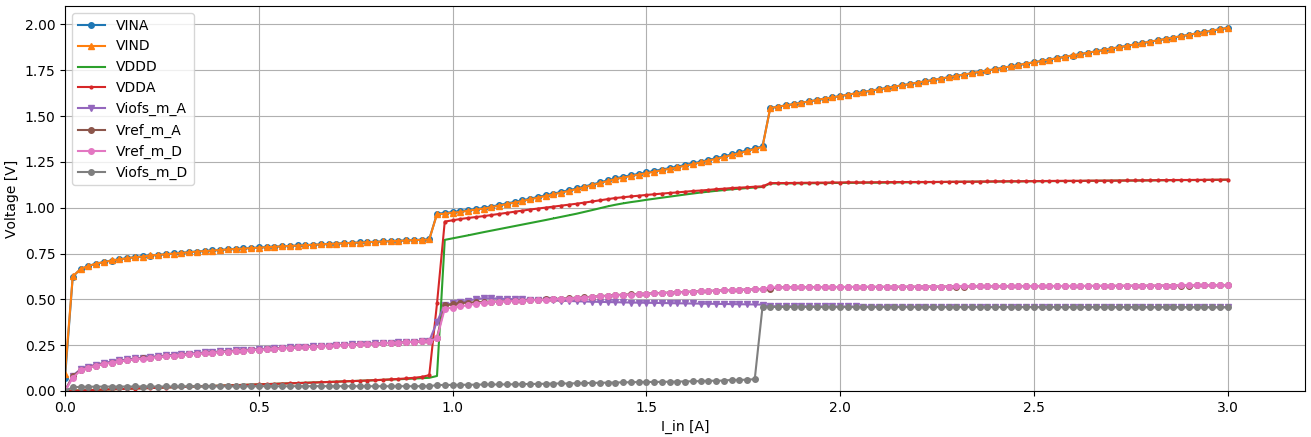
\includegraphics[width=\textwidth]{Immagini/PUI}
\caption{Grafico corrente-tensione ottenuto con i due regolatori in parallelo e variando la corrente da 0 A a 3.0 A, sull'asse x è riportata la corrente totale che poi si suddivide tra i due regolatori.}
\label{PUI}
\end{figure}
Come detto in precedenza, in RD53A, è stata lasciata la possibilità di tenere separate le alimentazioni dei due SLDO, mentre nella versione finale i due SLDO si troveranno in parallelo. 
In questa configurazione gli andamenti delle tensioni in ingresso (VINA e VIND) e di quelle in uscita (VDDD e VDDA) risultano migliori, nonostante gli offset di parte analogica e digitale si attivino in momenti diversi, come si può vedere in figura \ref{PUI}.
Questo miglioramento nel comportamento può essere attribuito all'utilizzo dell'alimentazione in parallelo dei due SLDO, poiché la corrente a disposizione si può suddividere in modo non uguale, come effettivamente accade. 
Lo sbilanciamento nella ripartizioni delle correnti ha inizio quando si 'attiva' $\mathrm{V_{iofs}}$ analogico e termina quando anche $\mathrm{V_{iofs}}$  digitale sale, come esplicitamente mostrato in figura \ref{CurrentSharing}.
%\begin{center}
%\begin{tabular}{|l|c|c|c|c|}
%\hline
% & \multicolumn{2}{c|}{Digitale} & \multicolumn{2}{c|}{Analogica} \\ \hline
% 
%& media & errore & media & errore \\ \hline
%
%$\mathrm{R_{eq}}$ & 0.7441 $\Omega$ & 0.0002 $\Omega$& 0.7396 $\Omega$ & 0.0009 $\Omega$ \\ \hline
%$\mathrm{V_{ofs}}$ & 0.8635 V& 0.003 V & 0.8688 V & 0.0011 V\\ \hline 
%\end{tabular}
%\end{center}

\begin{figure}
\centering
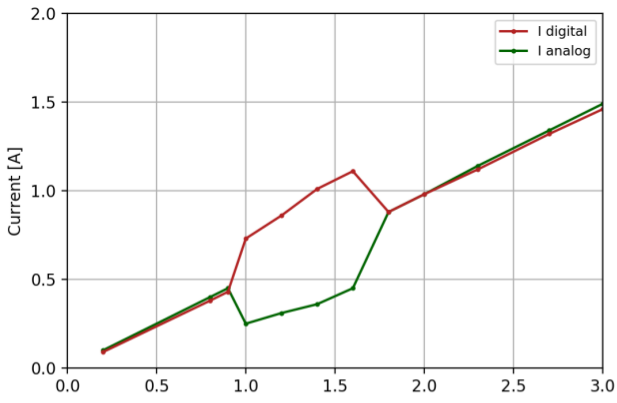
\includegraphics[scale=.4]{Immagini/CurrentSharing}
\caption{Misura della suddivisione della corrente tra i due regolatori posti in parallelo, sulle x è riportata la corrente totale fornita al parallelo.}%meeting del 16 aprile
\label{CurrentSharing}
\end{figure}
Il comportamento descritto è stato osservato anche in altri test e riportato in letteratura\cite{SLDO}. 
Lo sbilanciamento delle correnti avviene quando la tensione di uscita di uno dei due regolatori raggiunge la tensione di riferimento, mentre l'altro è ancora al di sotto del livello di riferimento. 
Nel momento in cui i due regolatori raggiungono un regime stabile, completando la fase di accensione, la distribuzione delle correnti torna ad essere bilanciata. 
Questo comportamento è noto e compreso: il meccanismo che lo innesca risiede nell'offset dell'amplificatore A2, utilizzato nel \textit{current mirror}. 
L'offset, infatti, implica un differente $\mathrm{V_{DS}}$ tra i transistor M1 e M2 influenzando il rapporto k nella regione lineare.
Dunque, fintantoché in uno dei due regolatori la tensione di uscita è minore di quella di riferimento, si ha uno sbilaciamento delle correnti. 
Quando viene raggiunto il livello di riferimento, M1 e M2 saturano e l'effetto dell'offset svanisce.

Questo problema, che si verifica durante l'accensione, può essere mitigato utilizzando particolari architetture con basso offset per l'amplificatore A2.

\subsubsection{Confronti fra le varie configurazioni}

Da ciascuna delle configurazioni, descritte nei paragrafi precedenti, sono stati ricavati, per la regione in cui il regolatore è attivo, offset e pendenza della curva caratteristica.
Idealmente ci aspettiamo che la pendenza sia confrontabile con R3 e l'offset con il doppio di $\mathrm{V_{iofs}}$.
A questo proposito ricordiamo che, per quanto riguarda i valori di default: 
\begin{center}
\begin{tabular}{lc}
\hline
$\mathrm{R3}$ & 600 $\Omega$ \\%misurata con il multimetro è 620
$\mathrm{V_{iofs}}$ & 0.500 V\\ 
\hline
\end{tabular}
\end{center}

In tabella \ref{table:results} sono riportati i valori di offset e pendenza dell'andamento caratteristico delle tensioni in ingresso per ciascuna configurazione.
Riguardo la configurazione è specificato se i due regolatori sono alimentati in parallelo o indipendentemente, se la corrente è stata fatta variare in modo crescente o decrescente e se le tensioni di riferimento per offset e per VDDD e VDDA sono prese internamente o fornite esternamente.

\begin{center}
\begin{table}
\begin{tabular}{|l|c|c|c|c|c|c|c|c|}
\hline
Regolatore & Alim. & Rampa & \multicolumn{2}{c|}{Vref [V]} & \multicolumn{2}{c|}{Voffset [V]} & Slope [$\Omega$] & Offset [V]\\ \hline
 
Analogico & \multirow{2}{*}{Indip.} & \multirow{2}{*}{Cres.} & Int. & - & Int. & - & 0.72 & 0.90 \\
Digitale  &  &  & Int. & - & Int. & - & 0.75  & 0.84 \\ \hline

Analogico & \multirow{2}{*}{Indip.} & \multirow{2}{*}{Decr.} & Int. & - & Int. & - & 0.71 & 0.90 \\
Digitale  &  &  & Int. & - & Int. & - & 0.73  & 0.86 \\ \hline

Analogico & \multirow{2}{*}{Indip.} & \multirow{2}{*}{Cres.} & Ext. & 0.550 & Int. & - & 0.75 & 0.87 \\
Digitale  &  &  & Ext. & 0.550 & Int. & - & 0.75  & 0.84 \\ \hline

Analogico & \multirow{2}{*}{Indip.} & \multirow{2}{*}{Cres.} & Int. & - & Ext. & 0.400 & 0.75 & 0.74 \\
Digitale  &  &  & Int. & - & Ext. & 0.400 & 0.79  & 0.68 \\ \hline

Analogico & \multirow{2}{*}{Paral.} & \multirow{2}{*}{Cres.} & Int. & - & Int. & - & 0.74 & 0.87 \\
Digitale  &  &  & Int. & - & Int. & - & 0.74  & 0.86 \\ \hline
\end{tabular}
\caption{Valore di offset e pendenza della curva caratteristica dei i due SLDO a seconda della configurazione.}
\label{table:results}
\end{table}
\end{center}

I risultati mostrati sono stati ottenuti mediando le varie misure effettuate con la stessa configurazione.
Queste risultano stabili all'interno di ciascun gruppo (variazioni inferiori ai 3 mV, tipicamente di 1 mV), mentre i valori medi, sia di R3 che di $\mathrm{V_{iofs}}$, variano fra una configurazione e l'altra.
%La prima cosa che si può notare è che i valori variano da una configurazione all'altra, mentre mantenendo per una stessa configurazione rimangono pressochè uguali, infatti i risultati sono stati ottenuti mediando su più misure.
Gli errori statistici relativi al fit lineare, da cui si ottengono Offset e Pendenza, sono trascurabili in confronto alle fluttuazioni date sia dall'utilizzo di una diversa configurazione, sia dalle possibili variazioni di temperatura nel tempo. 

\begin{figure}
\centering
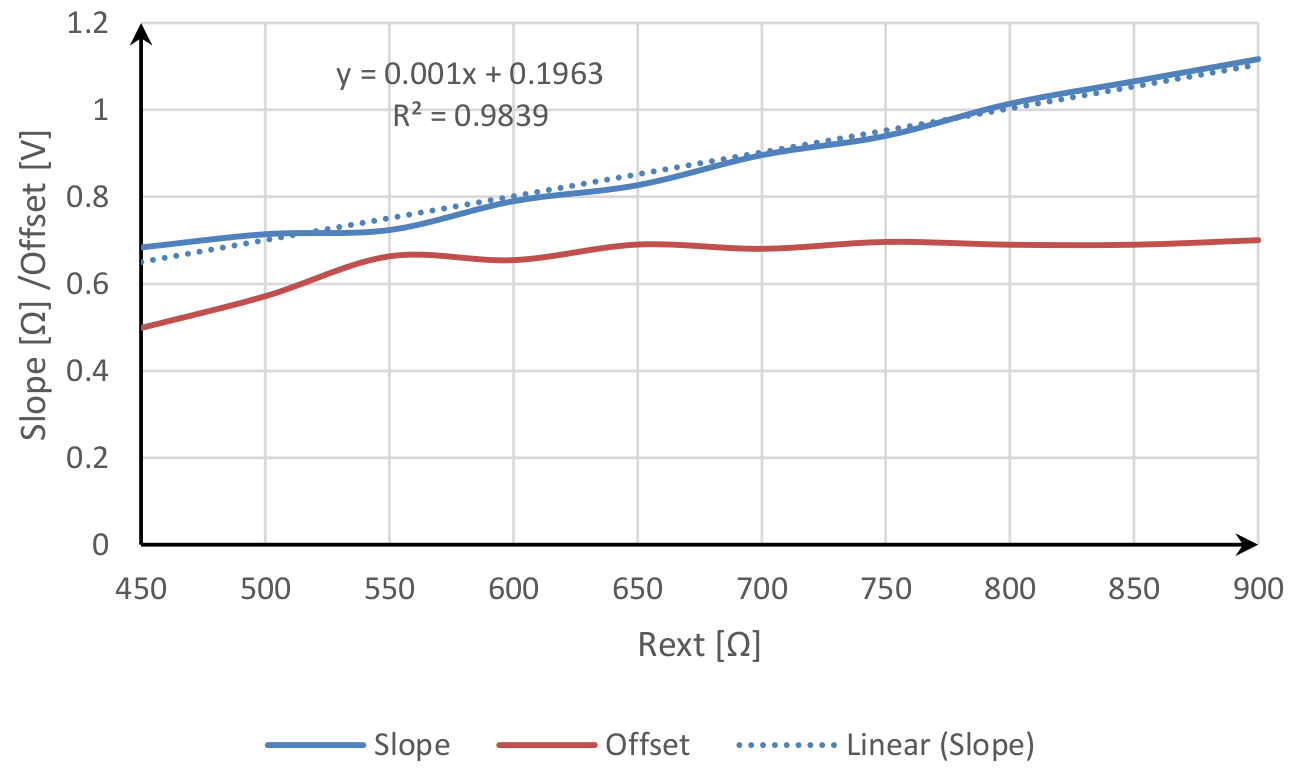
\includegraphics[width=\textwidth]{Immagini/R3Karagounis}
\caption{Andamento di offset e pendenza al variare della resistenza esterna utilizzata per definire la relazione tra $\mathrm{V_{in}}$ e $\mathrm{I_{in}}$.}%meeting del 13 aprile R^2 https://en.m.wikipedia.org/wiki/Coefficient_of_determination
\label{R3Karagounis}
\end{figure}

Dal confronto con i valori aspettati, inoltre, risulta evidente che la pendenza della retta caretteristica dello SLDO è sistematicamente maggiore e, viceversa, l'offset è sistematicamente minore. 
Questo comportamento è stato osservato anche in altri test eseguiti su chip da altri membri all'interno della collaborazione.
In particolare sono stati eseguiti test specifici al fine di comprenderne le cause. 
In figura \ref{R3Karagounis} è riportato l'andamento della pendenza e dell'offset al variare della resistenza R3
\footnote{
  \`E stata utilizzata una resistenza esterna regolabile.
}.
Per interpretare correttamente il grafico ricordiamo che, data la presenza nel circuito di un current-mirror con rapporto k = 1000, la pendenza della retta relativa a VIN nel grafico corrente-tensione sarà $\mathrm{\dfrac{R3}{k}}$. 
Dal fit lineare risulta che la relazione tra la resistenza esterna e la pendenza è $0.001x + 0.1963$, quindi k è effettivamente 1000, ma vi è una qualche resistenza spuria, in serie, del valore di circa 0.2 $\Omega$, che può variare da chip a chip. 
Questo test conferma il risultato ottenuto e giustifica la pendenza maggiore di quella aspettata. 
Per quanto riguarda l'offset e la sua sottostima, il fenomeno è di più difficile interpretazione.
In parte è dovuto alla differenza tra terra del chip e terra dello shunt?!.
\begin{figure}
\centering
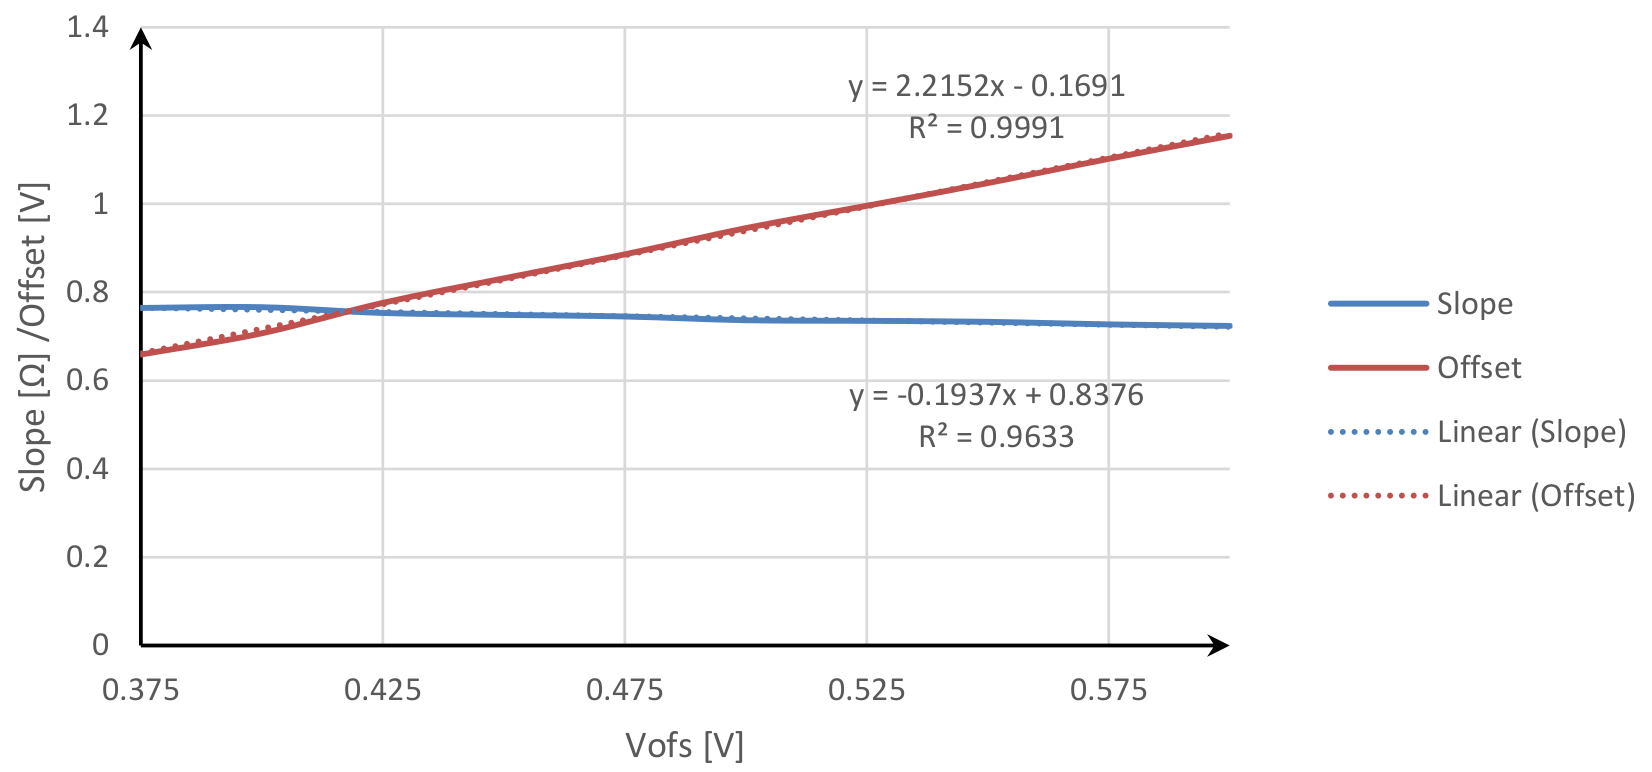
\includegraphics[width=\textwidth]{Immagini/OffsetKaragounis}
\caption{Andamento di offset e pendenza al variare della tensione di offset.}%meeting del 13 aprile
\label{OffsetKaragounis}
\end{figure}
Anche in questo caso sono stati compiuti test specifici riportati in figura \ref{OffsetKaragounis}. 
A differenza di quanto osservato con R3, l'offset non solo ha un andamento lineare con termine noto non nullo, ma possiede anche un fattore moltiplicativo maggiore di quello aspettato, i.e. 2. 
Infine, vi è una relazione tra offset e pendenza, su cui sono tutt'ora in corso studi per comprenderne le cause ed eliminarle.

\subsection{Variazioni di carico}

\begin{figure}
\centering
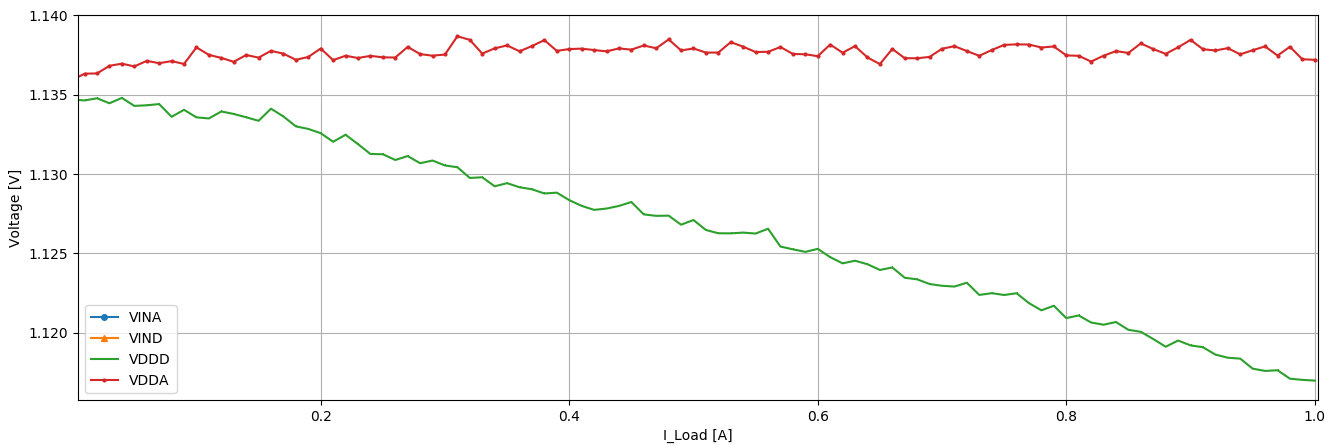
\includegraphics[width=\textwidth]{Immagini/LoadVDDD}
\caption{Andamento della tensione di alimentazione della parte analogica VDDA e digitale VDDD in funzione della corrente assorbita in più dal carico applicato allo SLDO digitale.}
\label{LoadVDDD}
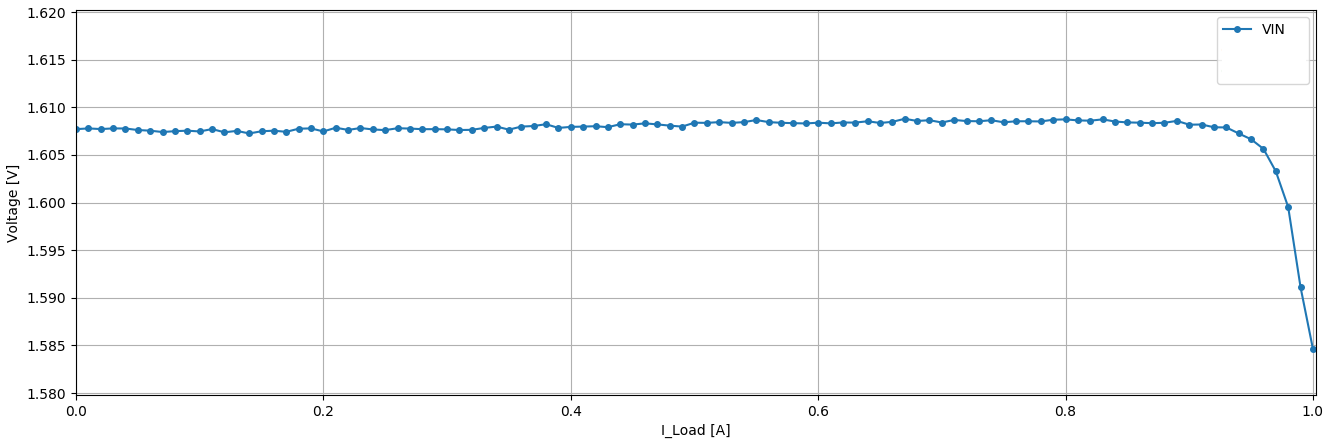
\includegraphics[width=\textwidth]{Immagini/LoadVIND}
\caption{Andamento della tensione di ingresso del chip in funzione della corrente assorbita in più dal carico applicato allo SLDO digitale.}
\label{LoadVIND}
\end{figure}

Per lo SLDO il carico è rappresentato dal chip, che fino a che si trova nella configurazione di default, ha consumi di corrente tipici pari a:
\begin{center}
\begin{tabular}{cc}
\hline
Regione Analogica & Regione Digitale \\ \hline
$\sim$0.400 A & $\sim$ 0.050 A\\ \hline     
\end{tabular}
\end{center}
Le misure riportate di seguito sono ottenute al variare del carico che applicato al VDDD/VDDA, ponendo in parallelo al chip un alimentatore Keithley utilizzato come sink di corrente. 
Come configurazione del chip si è utilizzato lo SLDO con i due circuiti di alimentazione in parallelo. 
La corrente in ingresso è stata fissata a 2 A, corrispondenti ad 1 A per ciascun SLDO. 
Dati i diversi consumi tra parte analogica e digitale, l'intervallo di variazione del carico è stato scelto diversamente per le due: tra 0 A e 1 Aper la parte digitale, tra 0 A e 0.69 A per l'analogica. 
Queste variazioni di carico non sono dinamiche, ma vanno considerate come statiche, infatti le tensioni di ingresso e di uscita vengono misurate, ad ogni incremento del valore del carico, su tempi scala lunghi rispetto a quelli di risposta del circuito di SLDO. 
Gli andamenti riportati di seguito vanno, quindi, interpretati come una deriva del valore della tensione prodotta dal regolatore in funzione dell'entità del carico. 
In figura \ref{LoadVDDD} sono mostrati gli andamenti ottenuti con il carico applicato alla parte digitale.
Come si può vedere, la tensione di alimentazione della regione digitale diminuisce gradualmente, arrivando ad una variazione di $\sim$18 mV per un carico addizionale di 1 A.
La parte analogica, invece, non risente di queste variazioni e rimane costante. %pendenza 18 mOhm(ogni 100 mA 1.8 mV
L'andamento della tensione in ingresso, figura \ref{LoadVIND}, ha invece una caduta di $\sim$24 mV che però si concentra nella parte finale partendo per valori di carico di circa 0.940 A.
Questo comportamento è plausibile se si considera che, da sola, la parte digitale consuma 50 mA e, dunque, la somma delle correnti assorbite tra chip e carico supera  quella a disposizione di 1 A. 
\begin{figure}
\centering
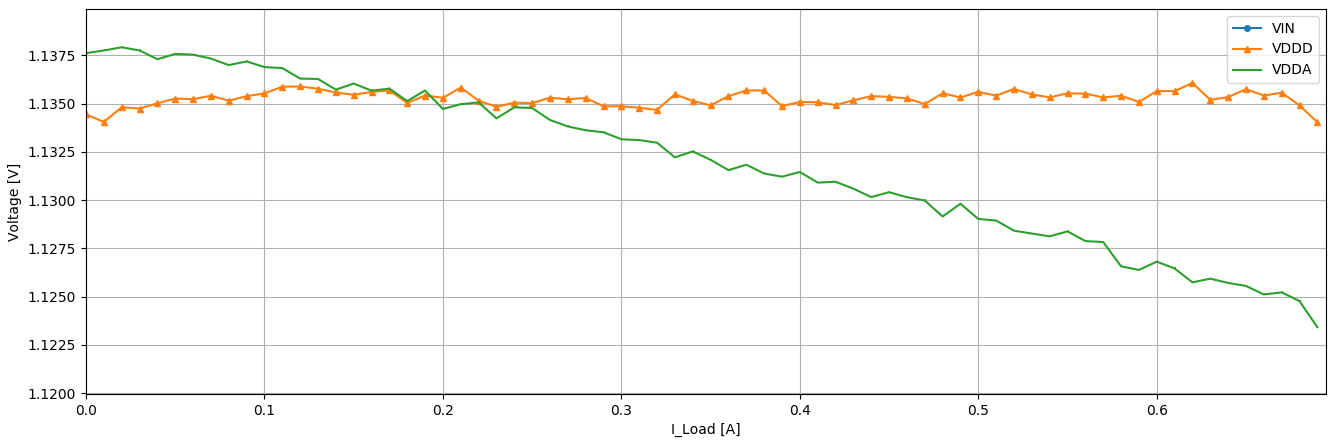
\includegraphics[width=\textwidth]{Immagini/LoadVDDA}
\caption{Andamento della tensione di alimentazione della parte analogica VDDA e digitale VDDD in funzione della corrente assorbita in più dal carico applicato allo SLDO analogico.}
\label{LoadVDDA}
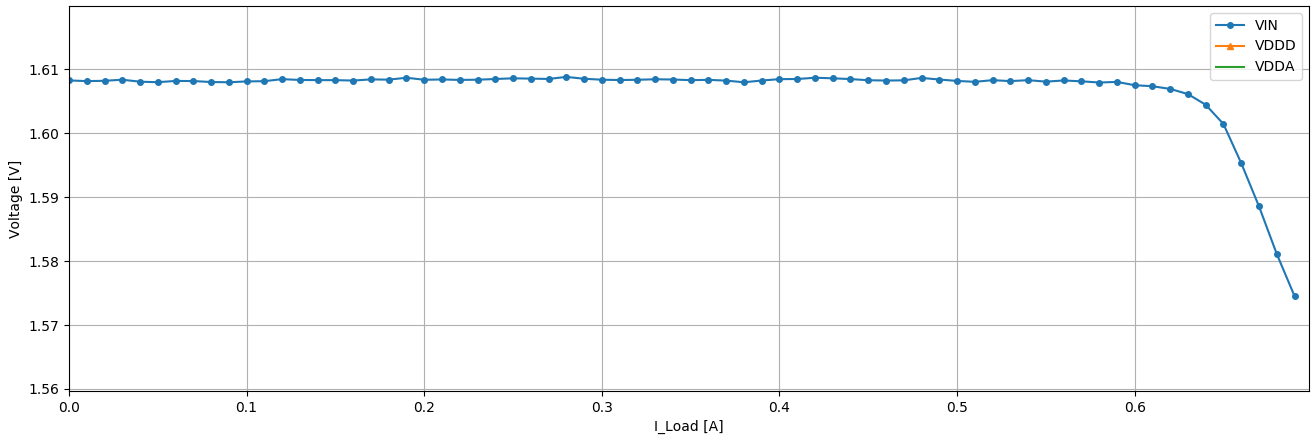
\includegraphics[width=\textwidth]{Immagini/LoadVINA}
\caption{Andamento della tensione di ingresso del chip in funzione della corrente assorbita in più dal carico applicato allo SLDO analogico.}
\label{LoadVINA}
\end{figure}
Un discorso analogo si può fare per la parte analogica, tenendo presente che i consumi minimi per il chip sono $\sim$400 mA.
L'andamento della tensione prodotta dal regolatore è riportata in figura \ref{LoadVDDA}, mentre, per quanto riguarda quella in ingresso il grafico di riferimento è quello di figura \ref{LoadVINA}. 
Per la tensione di uscita la caduta è di $\sim$15 mV per un carico di 0.690 A, %21mOhm
per quella in ingresso si ha, invece, una diminuzione di $\sim$26 mV in corrispondenza di un carico di 0.690 A, anche in questo caso il consumo totale di corrente supera 1 A. 
La diminuzione di tensione per $\mathrm{V_{in}}$ inizia con un carico di $\sim$0.610 A.

\subsection{Fast ramp-up}

\begin{figure}
\centering
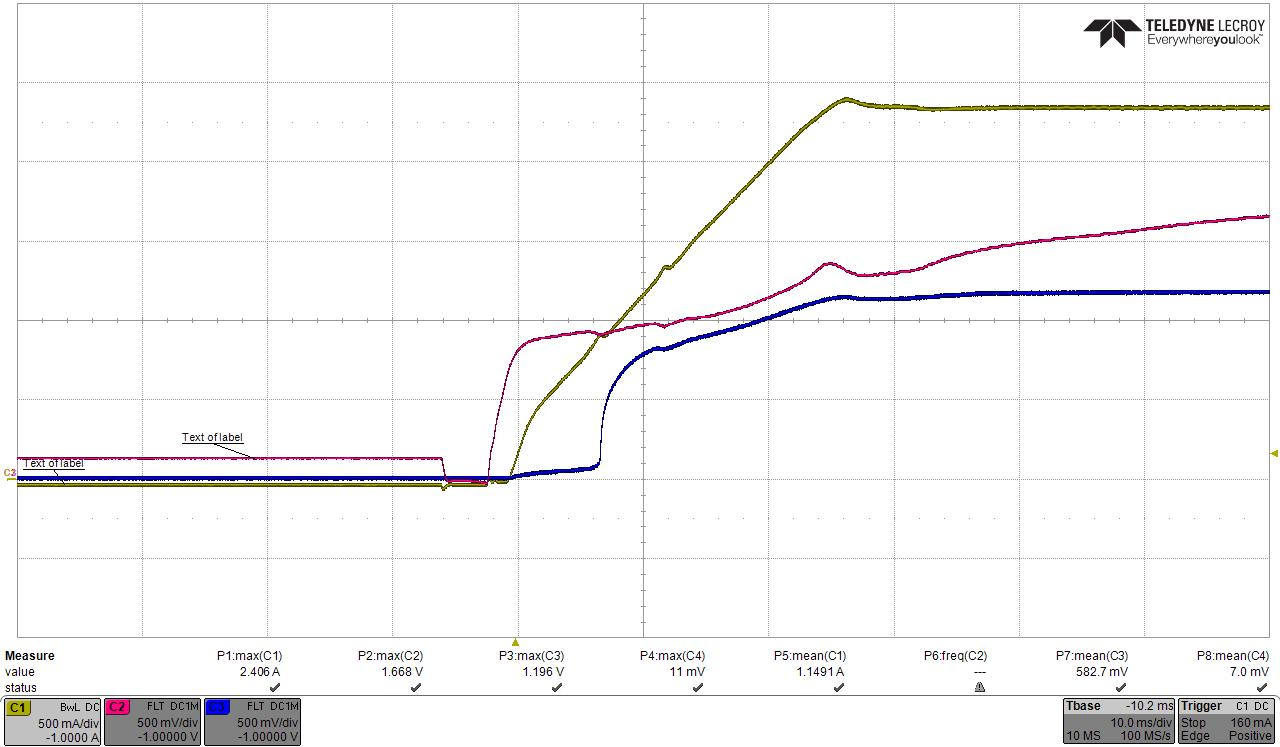
\includegraphics[scale=.3]{Immagini/rd-powup-dir6}
\caption{In giallo è riportata la corrente che in 25 ns passa da 0 A a 2.4 A, in fucsia la tensione in ingresso e in blu la tensione con cui è alimentata la parte digitale del chip VDDA.}
\label{rd-powup-dir6}
\end{figure}

\begin{figure}
\centering
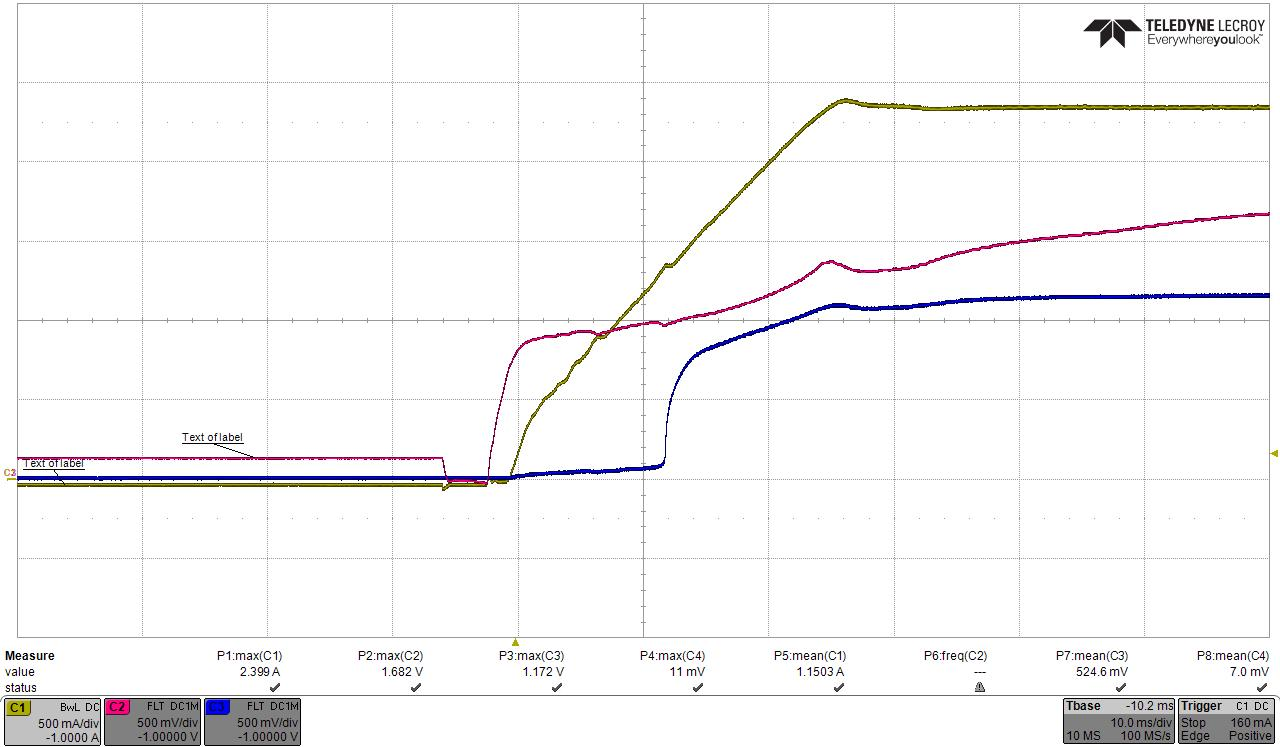
\includegraphics[scale=.3]{Immagini/rd-powup-dir7}
\caption{In giallo è riportata la corrente che in 25 ns passa da 0 A a 2.4 A, in fucsia la tensione in ingresso e in blu la tensione con cui è alimentata la parte analogica del chip VDDD.}
\label{rd-powup-dir7}
\end{figure}

Le misure riportate fino ad ora, sullo studio dei circuiti di SLDO in RD53A, sono da considerarsi statiche, in quanto sono ottenute su tempi scala lunghi in confronto a quello di risposta dello SLDO. 
%Fino ad ora gli scan sono stati eseguiti lentamente, in confronto al tempo di risposta del circuito di alimentazione, infatti tra un valore di corrente ed il successivo vi è quasi un secondo.
Inoltre, nel momento in cui il chip viene collegato ad un sistema di acquisizione dati, il consumo di regione, analogica e digitale, si modifica e, in base alle operazioni richieste, si hanno consumi variabili, che ci aspettiamo essee gestiti dal circuito di SLDO. 
Una fase particolarmente delicata, da questo punto di vista, è quella di accensione, poiché le variazioni di corrente sono i maggiori. 
Si è proceduto, quindi, ad eseguire scansioni in corrente passando da 0 A a 2.4 A in 25 ns con un incremento lineare. 
Anche in questo caso i due SLDO sono alimentati in parallelo, suddividendosi, quindi, la corrente erogata dal generatore. 
Come è possibile vedere dagli screenshoot dell'oscilloscopio, figure \ref{rd-powup-dir6} e \ref{rd-powup-dir7}, non sono presenti oscillazioni durante la fase di accensione.
La parte digitale e analogica non si attivano nello stesso momento, in particolare VDDD si accende dopo, in accordo con le misure precedenti.

% RIPARTIRE DA QUI
\section{Sviluppi}

Questi studi sull'alimentazione del chip si collocano in un più ampio progetto di sviluppo del nuovo tracciatore di fase due. In contemporanea a questi viene portato avanti lo sviluppo di sistemi di acquisizione dati in grado di dialogare con il chip e si stanno effettuando test sui tre \textit{front end} per studiarne la risposta sia prima che dopo processi di irraggiamento. 
In questo situazione lo sviluppo del circuito di alimentazione ha importanti legami con lo sviluppo del resto del chip, come detto il chip ha due regioni alimentate separatamente, digitale e analogica, questa scelta è dettata anche dalla necessità di proteggere la parte analogica, più sensibile, dal rumore della parte digitale. Se l'alimentazione fosse comune il rumore della parte digitale del chip andrebbe ad intaccare la parte analogica che è molto sensibile da questo punto di vista. 
Inoltre per operare una qualsiasi azione a livello di chip è necessario che lo stesso, una volta acceso, si trovi in una configurazione di default ben precisa, la corretta accensione è un problema legato al circuito di ShuntLDO, regione digitale e analogica devono attivarsi correttamente evitando oscillazioni durante il power-up e drop di tensione. 
Risulta quindi chiaro lo stretto legame che vi è tra alimentazione e sviluppo del chip. 

All'interno del lavoro di tesi è stato possibile anche un primo approccio allo sviluppo del sistema di acquisizione, in quanto lo studio riguarda oggetti attualmente in evoluzione essendo prototipi. L'approccio al sistema di DAQ rappresenta naturale in un'ottica di sviluppo del progetto di RD53A. A seguito diamo una breve descrizione del sistema di acquisizione utilizzato e dei primi risultati ottenuti su soglie di lettura e la relativa distribuzione di rumore. 



problemi legati a tensioni di riferimento troppo basse non riesce a dare Phase locked loop non sempre riesce, tensioni di otput troppo basse, causa dei vref bassi per problemi di progettazione dei circuiti di band gap, ma se non fa il pll nonn lo posso configurare a valori più alti.

\section{Sistema di acquisizione dati}
I sistemi di acquisizione dati che attualmente in sviluppo ma che è possibile utilizzare per eseguire alcuni test sono Yarr (\textit{Yet Another Rapid Readout}) \cite{YARR} e il sistema BDAQ sviluppato dall'Università di Bonn \cite{BDAQ}. 
%immagine sistema di acquisizione
Entrambi i istemi di acquisizione sfruttano fpga programmabili xilinx per il dialogo con il chip. 
Attraverso questi sistemi di acquisizione, sul cui sviluppo e le particolari caratteristiche non ci soffermeremo, non essendo questo il principale obbiettivo di questo lavoro di tesi, è possibile al momento vari test. 
In particolare riferendoci al sistema di acquisizione di Bonn i test più importanti, tra quelli attualmente disponibili, sono:
\begin{itemize}
\item \textbf{scan$\_$digital} Questo test semplicemente inietta un segnale digitale nei pixel abilitati per verificare la funzionalità della parte digitale del chip.%This basic scan injects a digital pulse into enabled pixels to test the digital part of the chip.
\begin{figure}
\centering
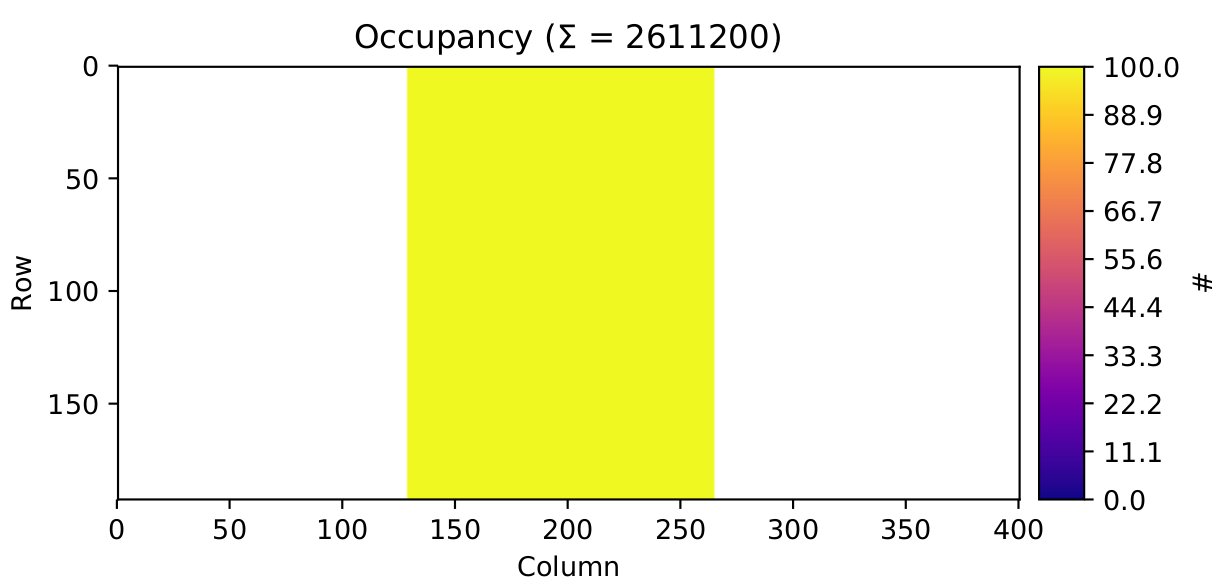
\includegraphics[width=\textwidth]{Immagini/ScanAnalogLinear}
\caption{Risultato del test \textbf{scan$\_$analog} sulla \textit{front end} lineare, tutti i canali di lettura hanno risposto il 100$\%$ delle volte.}
\label{ScanAnalogLinear}
\end{figure}
\item \textbf{scan$\_$analog}  Questo test è l'analogo di scan$\_$digital per la parte analogica. Un impulso con carica specifica viene iniettato nei canali di lettura abilitati in modo da verificare il funzionamento dei \textit{front end} analogici, figura \ref{ScanAnalogLinear}. %This basic scan injects a specified charge into enabled pixels to test the analog front-end. 
\item \textbf{scan$\_$threshold}  Questo test trova la soglia effettiva di ogni canale abilitato andando a iniettare segnali con carica via via crescente.%This script scans over different amounts of injected charge to find the effective threshold of the enabled pixels.
\item \textbf{meta$\_$tune$\_$threshold$\_$simple} Questo script effettua uno scan delle soglie per ogni possibile TDAC al fine di ottenere il valore ottimale per ogni pixel che consente di avvicinarsi alla soglia voluta. Il risultato di questo processo è un mask file.%This meta script simply performs a threshold scan for every possible TDAC to obtainthe optimal value per pixel to get as close to the target threshold as possible. The result is a TDAC mask file.
\end{itemize}
Altro file importante è il file contenente i parametri di configurazione dei registri \textbf{default$\_$chip.yaml}, che ogni volta che uno scan viene lanciato vengono scritti nel chip. 

Attraverso questi test è possibile, anche senza aver collegato un sensore al chip, controllare le funzionalità di parte analogica e digitale separatamente, analizzare la risposta dei tre \textit{front end} ad un segnale di calibrazione, ricavare una distribuzione delle soglie, la distribuzione del rumore e ottimizzare le soglie localmente (per \textit{front end} lineare e differenziale). 
A livello di questo lavoro di tesi risulta interessante esaminare il comportamento del circuito di alimentazione mentre il chip dialoga con il sistema di alimentazione così da avere informazioni su cosa accade quando ci sono variazioni nella corrente assorbita, senza dover simulare la cosa esternamente. 
Ad esempio durante il test scan$\_$threshold la parte analogica verifica il livello di soglia di ogni pixel andando a iniettare un segnale via via più grande nel circuito di lettura, in questa situazione è corretto pensare che ci siano variazioni nella corrente assorbita anche grandi. 
Una prima prova che è interessante eseguire consiste nel confrontare una situazione in cui è utilizzato il regolatore con lo Shunt e una situazione in cui non è utilizzato lo Shunt e il chip è alimentato in configurazione LDO. In seguito è lecito chiedersi se, effettivamente in una catena seriale di due chip l'attivita di uno non influenza l'altro. Cioè se il circuito di SLDO riesce ad nascondere al chip eventuali fluttuazioni e rumore  che vi sono nella catena.

\subsubsection{LDOvsSLDO}
\begin{figure}
\centering
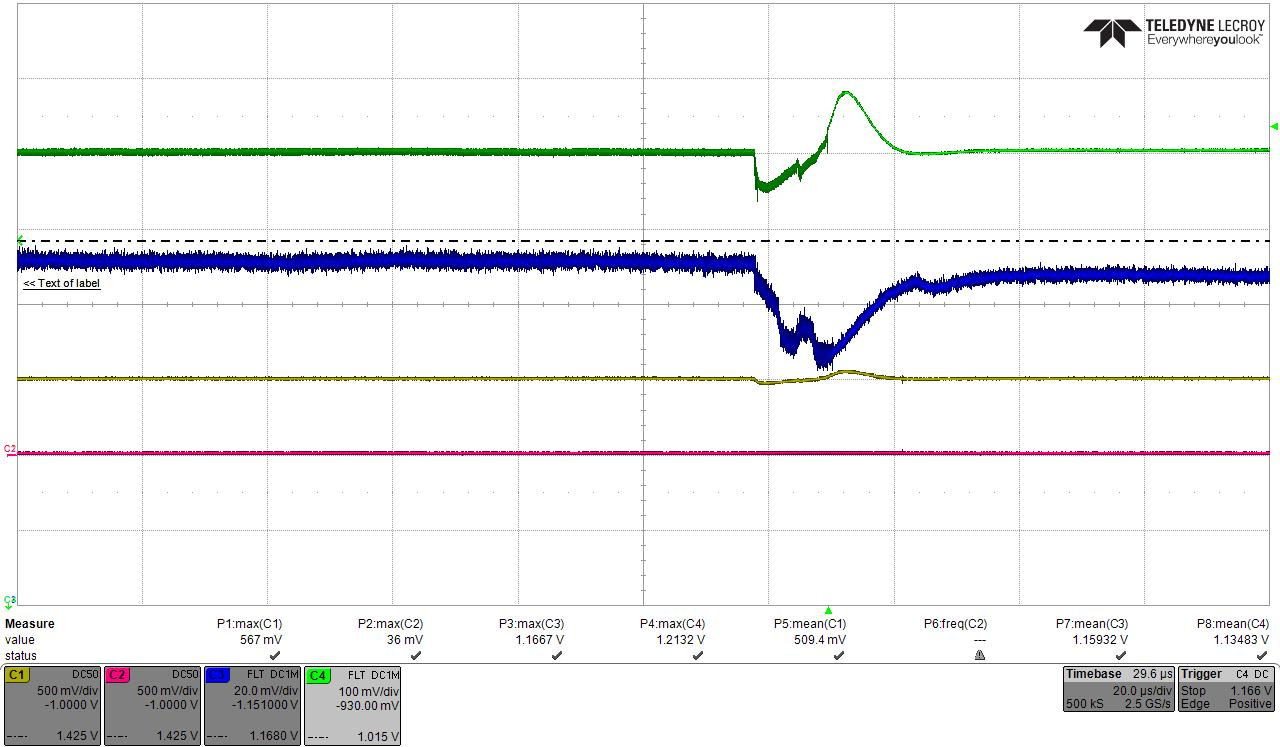
\includegraphics[scale=.3]{Immagini/alllin1}
\caption{VDDD in verde con scala 100 mV/div., e VDDA, in blu con scala 20 mV/div.}
\label{alllin1}
\end{figure}
\begin{figure}
\centering
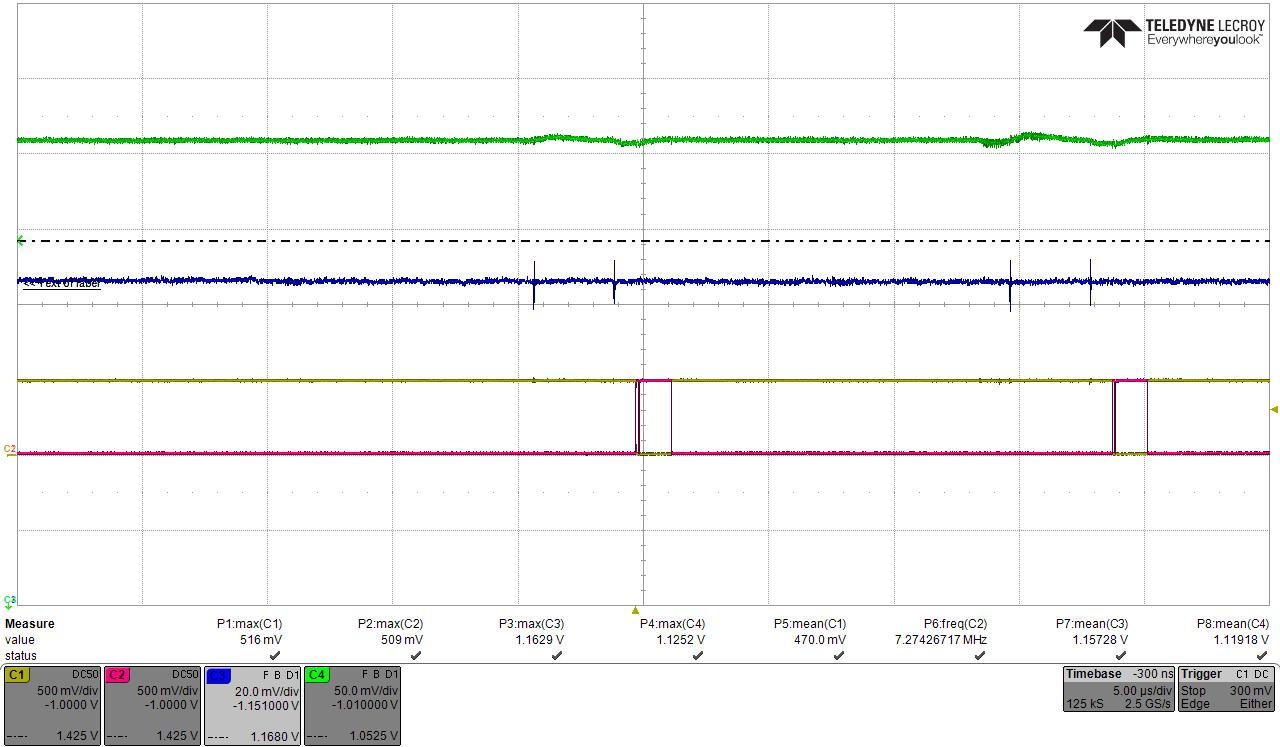
\includegraphics[scale=.3]{Immagini/alllin2}
\caption{VDDD in verde con scala 50 mV/div., e VDDA, in blu con scala 20 mV/div.}
\label{alllin2}
\end{figure}
Riportiamo di seguito una misura che aiuta a capite quali siano i vantaggi effettivi di utilizzare un circuito di alimentazione che implementi uno Shunt oltre al regolatore. Quello che è stato fatto è monitorare le tensioni di alimentazione del chip, VDDD e VDDA, mentre attraverso il sistema di acquisizione dati veniva richiesto al chip di eseguire il test scan$\_$threshold\footnote{Per cercare di massimizzare gli effetti è stato aumentato il numero di pixel uin cui veniva iniettato contemporaneamente un segnale, anch'esso preso molto grande}. 
In questo modo è stato possibile verificare cosa accade con variazioni di carico prorpie dell'attività del chip, senza doverle simulare esternamente. 
Dal confronto tra i risultati ottenuti in configurazione con o senza shunt è emersa chiaramente l'importanza di questo elemento, non solo per evitare cheun malfunzionamento del chip renda inutilizzabile tutta la catena, ma anche per rendere stabili le tensioni generate dal regolatore. 
In figura \ref{alllin1} sono riportate le tensioni VDDD e VDDA in questo caso è stato scelto di utilizzare il chip senza Shunt (alimentato in tensione) e durante il dialogo con il sistema di acquisizione si sono verificate variazioni notevoli nelle tensioni. (per rendere il tutto estremo iniezione di carica su più canali) Con le stessse condizioni utilizzando lo shunt gli sbalzi di tensione sono pressochè spariti (alimentato in corrente), vedi figura \ref{alllin2}, questo perché le variazioni di carico in presenza dello shunt sono gestite localmente, mentre in modalità LDO l'alimentazione è in tensione ed è il generatore esterno che adatta la corrente erogata ai consumi del chip.

%\begin{figure}
%\centering
%\includegraphics[scale=.3]{Immagini/}
%\caption{.}
%\label{}
%\end{figure}

\subsubsection{BDAQ}
\begin{figure}
\centering
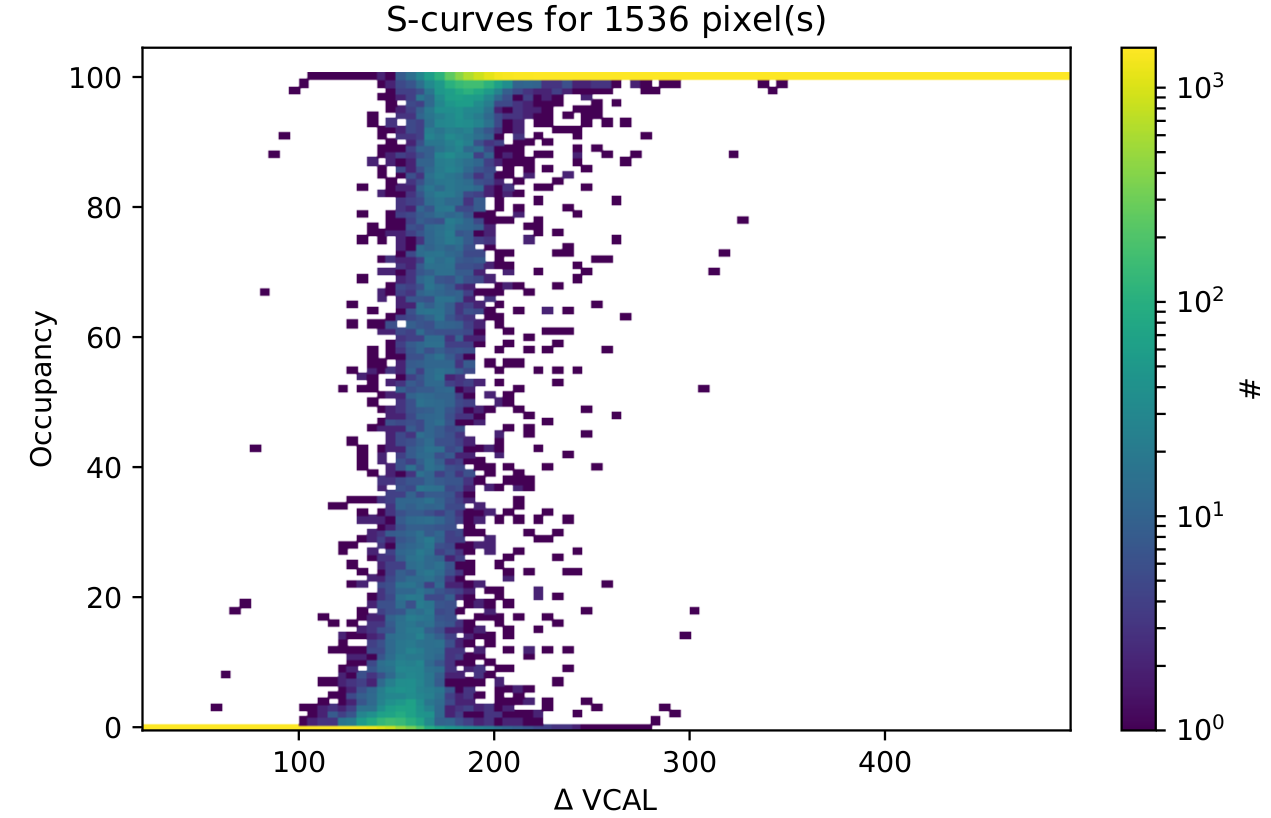
\includegraphics[width=0.9\textwidth]{Immagini/Scurves}
\caption{Risultato del test \textbf{scan$\_$threshold}. Sulle x vi è il valore in unitàarbitrarie dell'ampiezza del segnale iniettato nel canale di lettura, sulle y vi è il numero di volte che si è avuto risposta e la scala di colore è il numero di canali.}
\label{Scurves}
\end{figure}
\begin{figure}
\centering
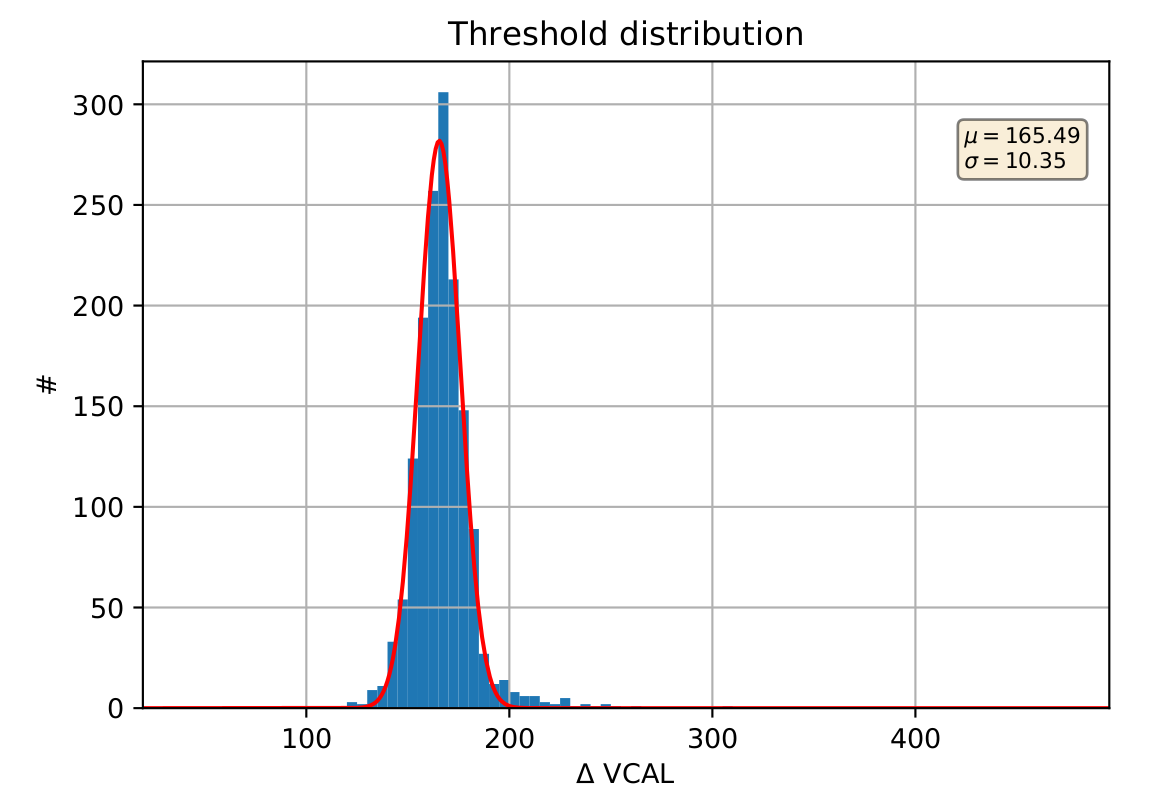
\includegraphics[width=0.75\textwidth]{Immagini/Threshold}
\caption{Distribuzione della soglia ottenuta dalle S-curves.}
\label{Threshold}
\end{figure}
Prima di procedere con la presentazione dei risultati è necessario dare almento un'idea guida di che operazione vengono eseguite durante lo scan delle soglie al fine di comprendere meglio il significato delle varie distribuzioni.
Attraverso i parametri di configurazione è possibile decidere una soglia globale uguale per tutti i canali di lettura, nella pratica però la soglia varierà leggermente tra un canale e l'altro. 
Quello che si avrà sarà una distribuzione delle soglie intorno ad un valore centrale, oltre a questa dispersione delle soglie, a causa del rumore, si avrà che la risposta del circuito di lettura non sarà una theta in funzione della carica raccolta. 
Alle volte il rumore si sommerà al segnale facendo rispondere il discriminatore anche a segnali più piccoli della soglia. Se sul ciascun canale iniettiamo un segnale via via più grande ripetendo il processo più volte e andando a riportare quante volte si ha risposta in funzione del segnale iniettato si ottengono le così dette Scurves, se non ci fosse rumore si avrebbe un gradino. 
Per ogni canale si ha una Scurve messe tutte insieme danno un grafico come quello riportato in figura \ref{Scurves}, dove il colore indica quanti sono i pixel che a un dato Vcal si sono accesi un dato numero di volte. Dal fit della singola Scurves si ricava un valore di soglia e rumore, mettendo insieme i risultati per tutti i canali si ottengolo le distribuzioni delle stesse, in figura\ref{Threshold} è riportata la distribuzione delle soglie. 
\begin{figure}
\centering
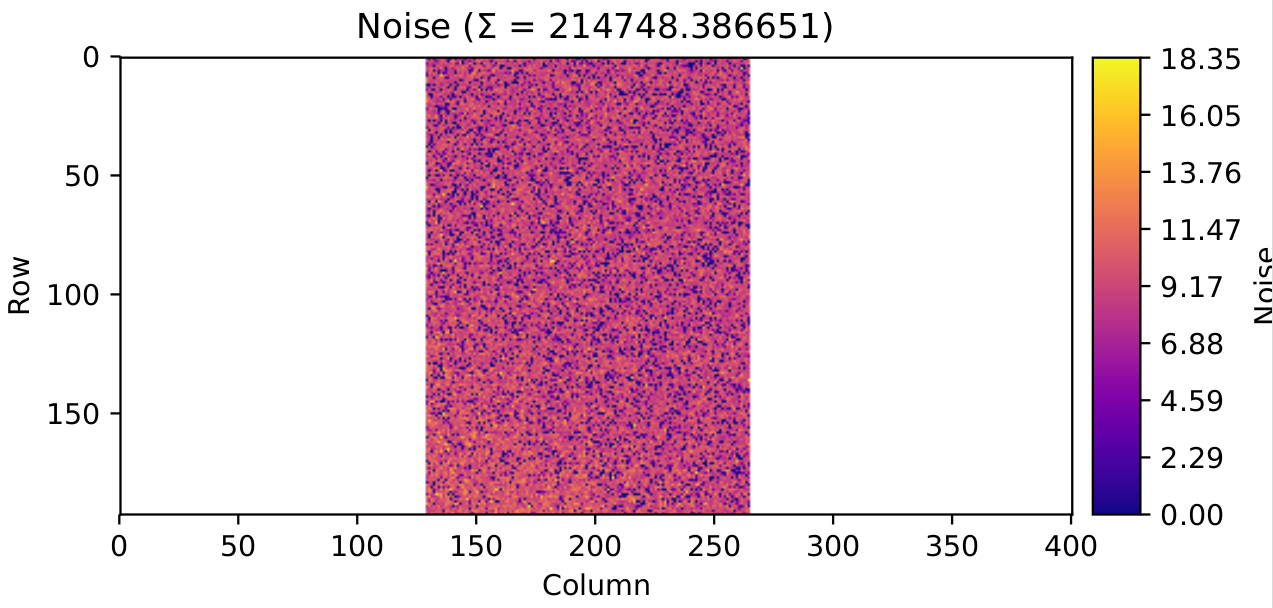
\includegraphics[width=0.9\textwidth]{Immagini/NoiseMap}
\caption{Mappa del livello di rumore pixel per pixel del FE lineare.}
\label{NoiseMap}
\end{figure}
Oltre alle distribuzioni di soglia e rumore il test restituisce anche una mappa per ogni pixel di questi, questo è utile per verificare se la risposta è omogenea o se per qualche motivo ci sono effetti tali che alcune zone risultano più rumorose, in figura \ref{NoiseMap} è riportata la mappa del rumore ottenuta per il \textit{front end} lineare. 
La soglia è il livello minimo a cui l'elettronica risponde, se non ci fosse rumore le S-curves sarebbero gradini, nella realtà a causa del rumore che si somma al segnale questi gradini ideali diventano curve, meno assomiglia ad un gradino maggiore è il rumore.
Come detto in precedenza l'utilizzo dello SLDO dovrebbe evitare il propagarsi del rumore tra parte analogica e digitale(visto che usano due shuntLDO diversi), ma anche evitare che disturbi della linea vengano visti dal carico. 
\begin{figure}
\centering
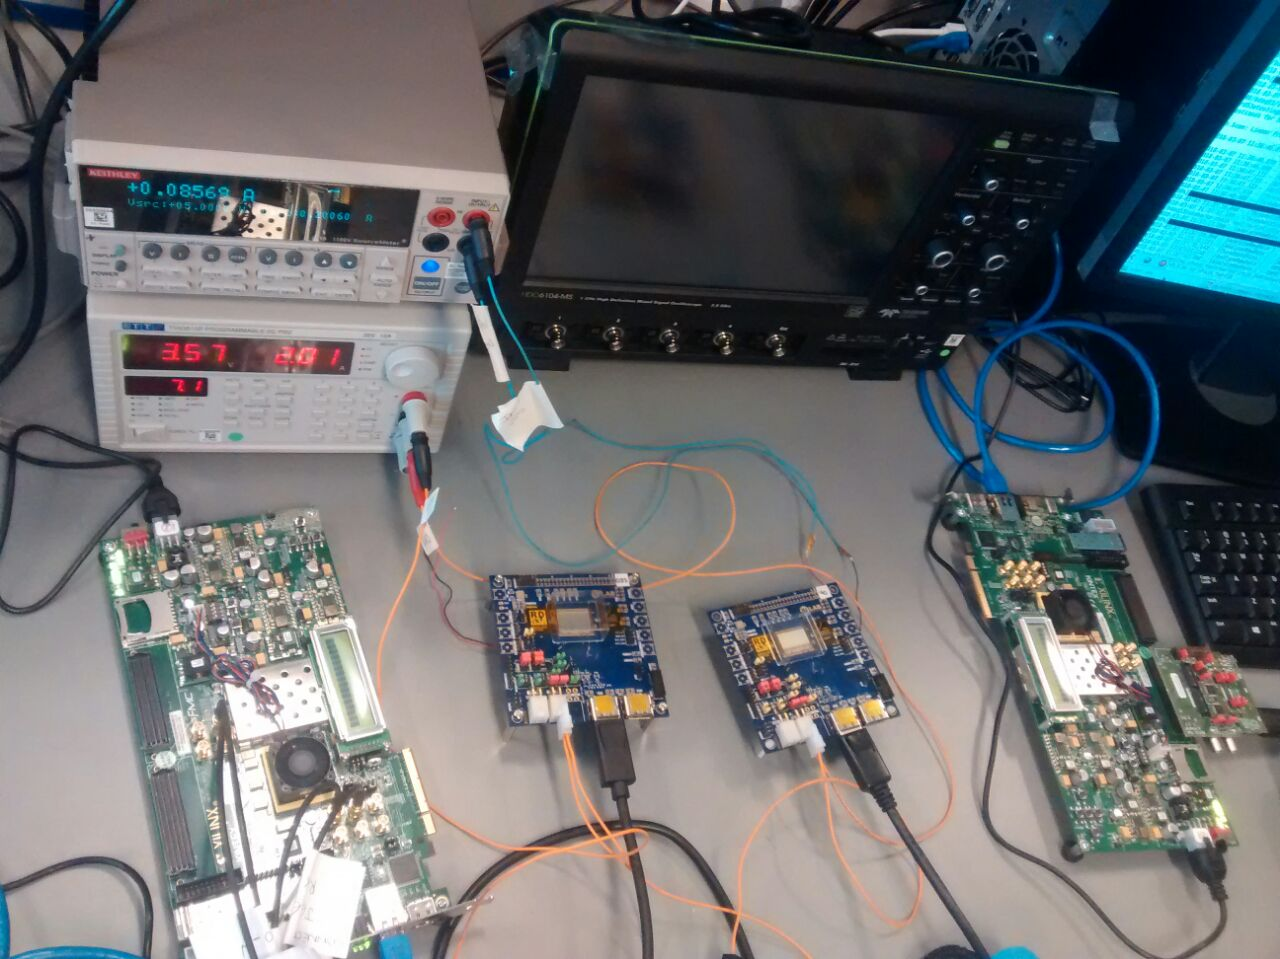
\includegraphics[width=0.75\textwidth]{Immagini/chipserial}
\caption{Fotografia del setup, i due chip posti sulla Single Chip Card sono al centro e ognuno di essi è collegato a una fpga che gestisce la comunicazione tra RD53A e il computer.}
\label{chipserial}
\end{figure}
Al fine di verificare se vi è una correlazione tra la ditribuzione del rumore e l'utilizzo del chip all'interno di una catena seriale si è proceduto con il mettere a confronto i risultati ottenuti da test eseguiti prima con il chip singolo e poi mettendone due in serie o in parallelo. 
In figura \ref{chipserial} è riportata un'immagine del setup. 
Tutte e tre le misure sono state eseguite utilizzando la configurazione di SLDO.  

Le misure riportate fanno riferimento solo al \textit{front end} lineare, in quanto al momento della presa dati era quello su cui era possibile lavorare meglio, sia a livello di ottimizzazione dei vari parametri, sia a livello di software.
I risulati sono riportati in funzione di VCAL, parametro dello scan, la cui conversione in elettroni è 1:10, per una u.a. corrispondono 10 $\mathrm{e^{-}}$.

\begin{figure}[h]
\centering
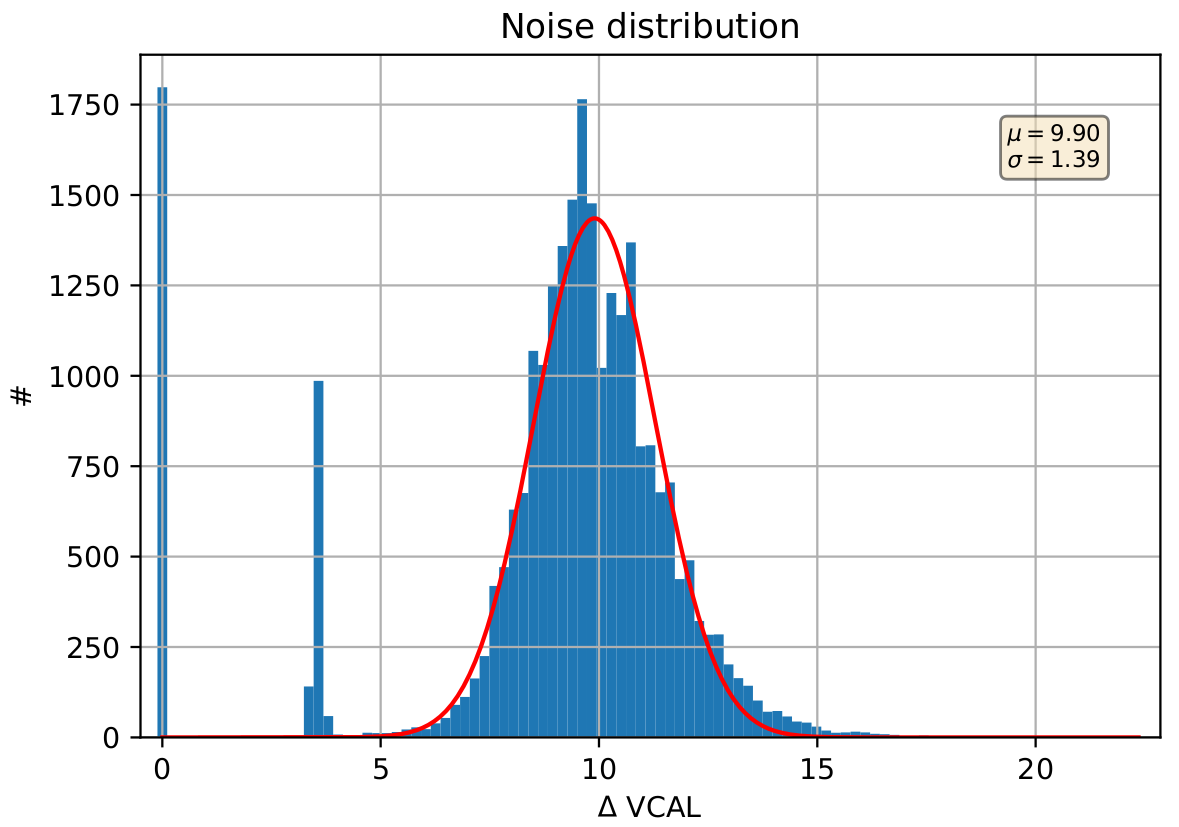
\includegraphics[width=0.75\textwidth]{Immagini/NoiseSingle}
\caption{Distribuzione di rumore ottenuta attraverso il test di \textbf{scan$\_$threshold} su un chip alimentato singolarmente.}
\label{noisesingle}
\end{figure}
\begin{figure}
\centering
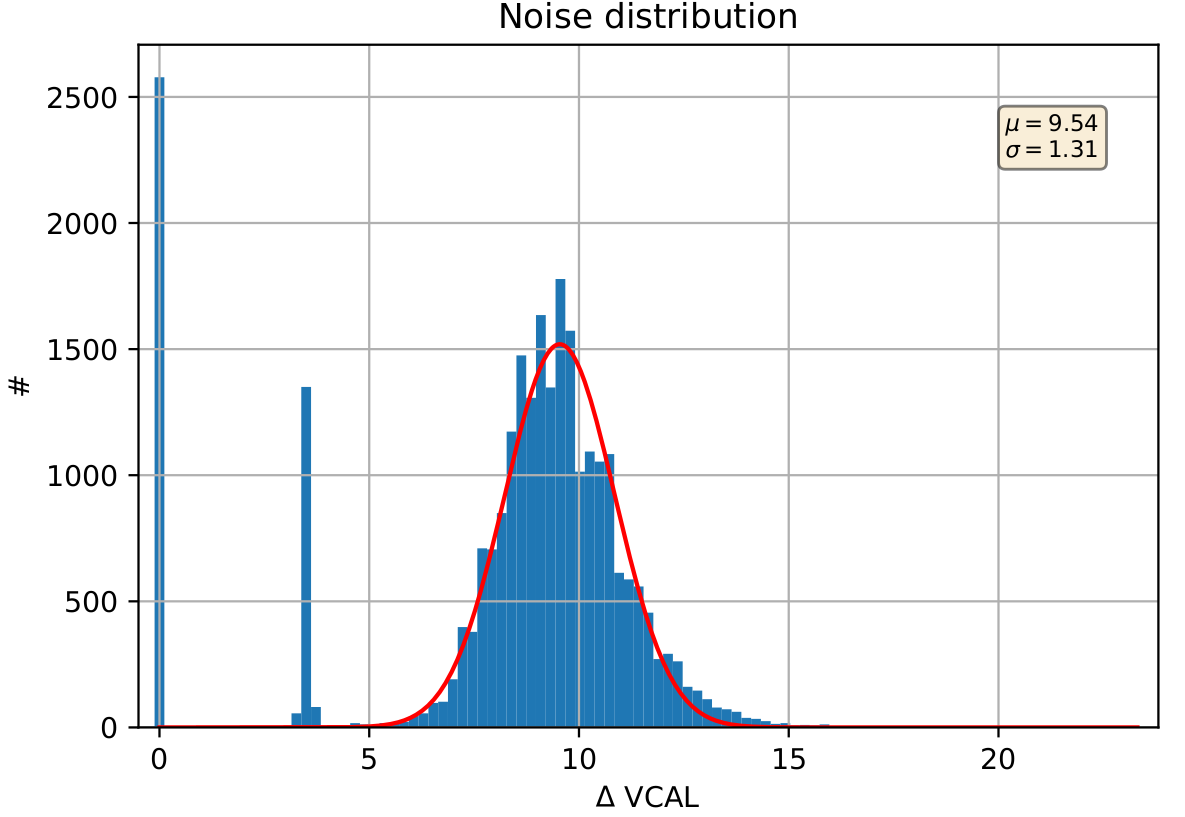
\includegraphics[width=0.75\textwidth]{Immagini/NoiseSerial}
\caption{Distribuzione di rumore ottenuta attraverso il test di \textbf{scan$\_$threshold} su un chip alimentato in serie ad un secondo, anche sul secondo chip sono stati eseguite scansioni in contemporanea.}
\label{noiseserial}
\end{figure}

Trascurando i risultati relativi alla distribuzione delle soglie, che sono indipendenti dalla distribuzione del rumore, riportima in figura le distribuzioni ottenute per il rumore nei tre casi:
\begin{itemize}
\item Chip singolo, figura \ref{noisesingle}.
\item Serie di due chip, figura \ref{noiseserial}.
\item Parallelo di due chip, figura \ref{noiseparallel}.
\end{itemize}
Come si puòvedere nonostante nel caso serie e parallelo anche sul secondo chip fossero eseguiti test, in modo da simularne un'attività, la distribuzione del rumore non peggiora. 
Questo dimostra che effettivamente esternamente i chip non sono visibili e viceversa il chip non vede le variazioni che ci sono sulla linea.

\begin{figure}
\centering
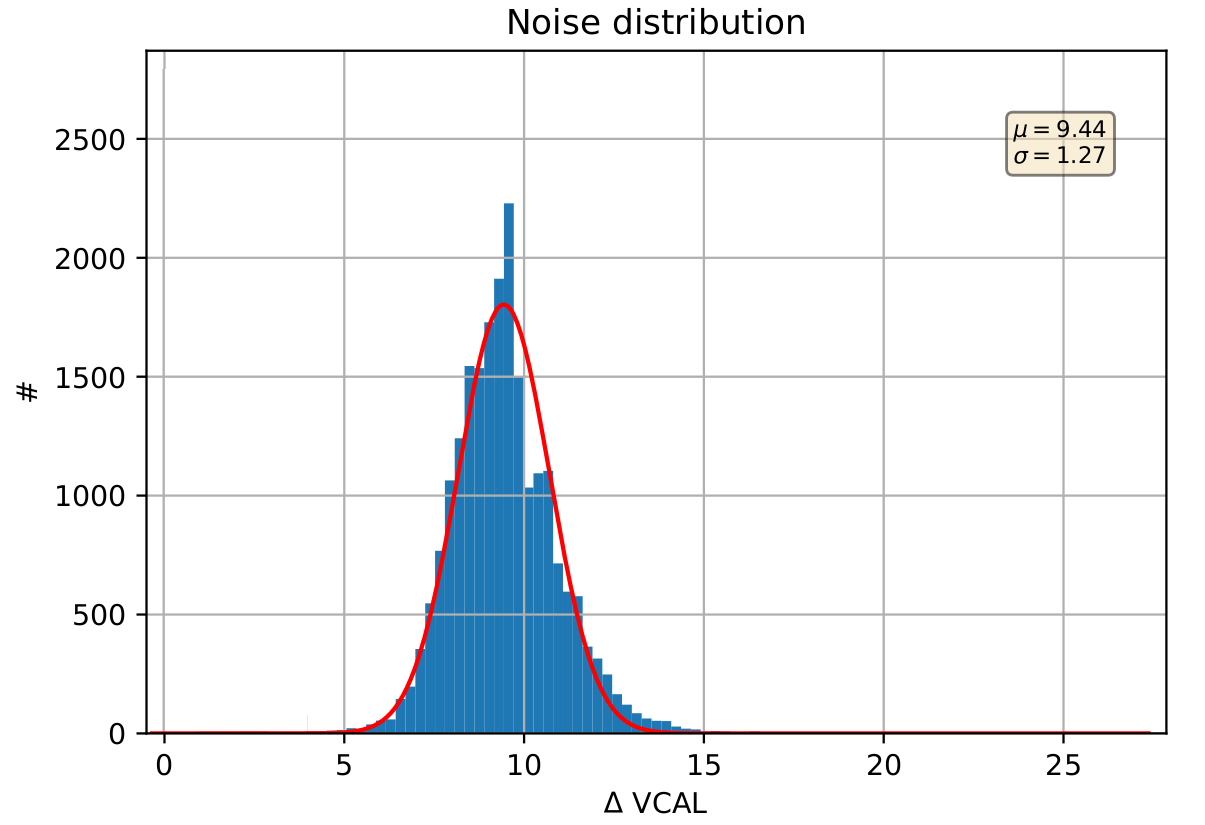
\includegraphics[width=0.75\textwidth]{Immagini/NoiseParallel}
\caption{Distribuzione di rumore ottenuta attraverso il test di \textbf{scan$\_$threshold} su un chip alimentato in parallelo ad un secondo, anche sul secondo chip sono stati eseguite scansioni in contemporanea.}
\label{noiseparallel}
\end{figure}
